%latexmk -pdf -pvc Notes
\documentclass{article}
\setlength{\oddsidemargin}{6pt}
\setlength{\textwidth}{440pt}
\vspace{-8ex}
\usepackage{mathtools}
\usepackage{enumitem}
\DeclarePairedDelimiter{\ceil}{\lceil}{\rceil}
\usepackage{listings}
\usepackage{amsmath}
\usepackage{color}
\usepackage{graphicx}
\usepackage[left=0.70in, right=0.70in, top=0.50in, left=0.70in, headsep=0pt]{geometry}
\graphicspath{ {./assets/} }

\definecolor{dkgreen}{rgb}{0,0.6,0}
\definecolor{gray}{rgb}{0.5,0.5,0.5}
\definecolor{mauve}{rgb}{0.58,0,0.82}

\lstset{frame=tb,
  language=Java,
  aboveskip=3mm,
  belowskip=3mm,
  showstringspaces=false,
  columns=flexible,
  basicstyle={\small\ttfamily},
  numbers=none,
  numberstyle=\tiny\color{gray},
  keywordstyle=\color{blue},
  commentstyle=\color{dkgreen},
  stringstyle=\color{mauve},
  breaklines=true,
  breakatwhitespace=true,
  tabsize=3
}

\title{CMSC420 Advanced Data Structures}
\date{}
\begin{document} 
  \author{Michael Li}
  \title{CMSC420 Advanced Data Structures}
  \maketitle
  \tableofcontents
  \newpage
  \noindent \section{Lists}
  \begin{lstlisting}
    init() // initializes list
    get(i) // returns element at index i
    set(i, x) // sets ith element to x
    length() // returns number of elements in the list
    insert(i, x) // insert x prior to element a_{i} (shifts indices after)
    delete(i) // deletes ith element (shift indices after)
  \end{lstlisting}
  Sequential Allocation (Array): when array is full, increase  its size but a constant factor (e.g. 2). Amortized array operations still O(1) \\ \\
  Linked Allocation (Linked List) \\ \\
  Arrays and LinkedLists can be used to create:
  \begin{itemize}[noitemsep]
  \item Stack(push, pop): on on end of the list
  \item Queue(enqueue, dequeue): insert at tail (end) and remove from head (start)
  \item Deque(combo stack and queue): can isnert and remove from either ends of list
  \item Multilist: multiple lists combined 1 aggregate structure (e.g. ArrayList)
  \item Sparse Matrix: create 2n linked lists for each row and col
    \setlist{nolistsep}
    \begin{itemize}[noitemsep]
      \item Each entry stores a row index, col index, value, next row ptr, and next col ptr
    \end{itemize}
  \end{itemize}
  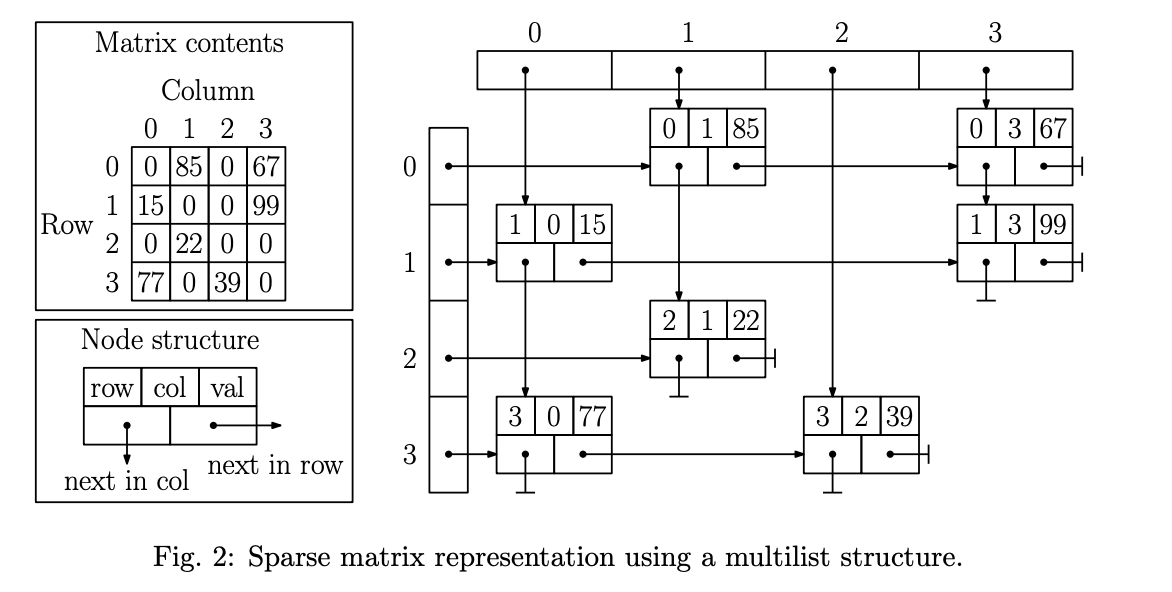
\includegraphics[width=\textwidth]{Fig_2}
  \newpage
  \noindent\section{Trees}
  Free Tree: connected, undirected graph with no cycles (like MST)\\ \\
  Root Tree: each non-leaf node has $\geq$ 1 children and a single parent (except root)\\
  \setlist{nolistsep}
  \begin{itemize}[noitemsep]
  \item Aborescence = out-tree \quad Anti-arborescence = in-tree 
  \item Depth = max \# of edges of path from root to a node \\
  \end{itemize}
  One way to represent a tree is to have a pointer to first child and then a pointer to next sibling \\ \\
  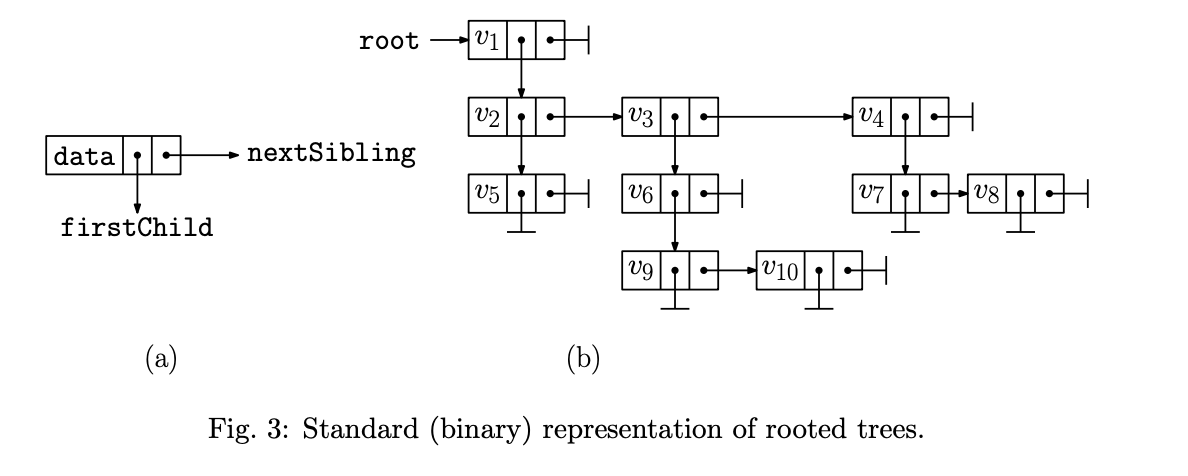
\includegraphics[width=\textwidth]{Fig_3}
  Binary Tree: rooted, ordered tree where each non-leaf node has 2 possible children (left, right)
  \setlist{nolistsep}
  \begin{itemize}[noitemsep]
  \item Full Tree: All nodes either have 0 children or 2 children
  \item Can make full binary tree by extending tree by adding external nodes to replace all empty subtrees
  \end{itemize}
  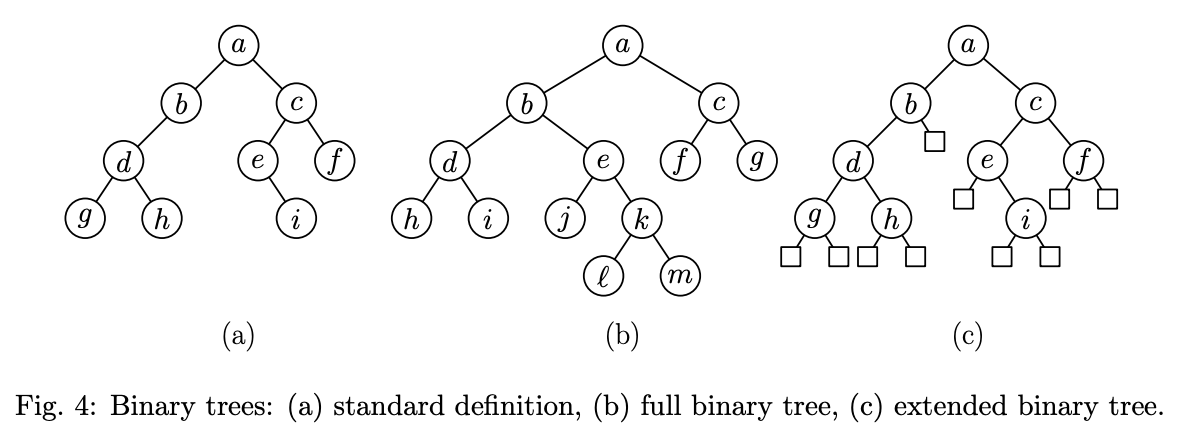
\includegraphics[width=\textwidth]{Fig_4}
  \begin{lstlisting}
    class BinaryTreeNode<E> {
      private E entry;
      private BinaryTreeNode<E> left;
      private BinaryTreeNode<E> right;
      ...
    }
  \end{lstlisting}
  \newpage
  \noindent In-order traversal: left, root, right \\
  Pre-order traversal: root, left, right \\ 
  Post-order traversal: left, right, root\\ \\
  If there are n internal nodes in an extended tree, there are n+1 external nodes
  \setlist{nolistsep}
  \begin{itemize}
  \item Proof by induction: Extended tree binary tree with n internal nodes has n+1 external nodes has 2n+1 total nodes
  \item Let x(n) = number of external nodes given n internal nodes and prove x(n) = n + 1
  \item Base Case x(0) = 1 a tree with no internal nodes has 1 external node
  \item IH: Assume x(i) = i + 1 for all i $\leq$ n - 1
  \item IS: let $n_{L}$ and $n_{R}$ be the number of nodes in Left and Right subtrees
  \item x(n) = ($n_{L}$ + 1) + ($n_{R}$ + 1) = (1 + $n_{L}$ + $n_{R}$) + 1 = n + 1 external nodes
  \item so n + 1 (external) + n (internal) = 2n + 1
  \item Moreover, about 1/2 of nodes of extended Binary Tree are leaf nodes \\
  \end{itemize}
  Threaded Binary Tree: Give null pointers information about where to traverse next
  \setlist{nolistsep}
  \begin{itemize}
  \item If left-child = null then stores reference to node's inorder predecessor
  \item If right-child = null then stores references to node's inorder successor
  \end{itemize}
  \includegraphics[width=\textwidth]{Fig_6}
  \begin{lstlisting}
    BinaryTreeNode inOrderSuccessor(BinaryTreeNode v) {
      BinaryTreeNode u = v.right;
      if(v.right.isThread) return u;
      while(!u.left.isThread) u = u.left;
      return u;
    }
  \end{lstlisting}
  \begin{itemize}[noitemsep]
  \item If v's right-child is a thread, then we follow thread.
  \item Otherwise go through v's right child and iterate through left-child links until we find the last node before the thread\\
  \end{itemize}
  Complete Binary Tree: represented using sequential allocation (array) because no space is wasted 
  \begin{itemize}[noitemsep]
  \item number of nodes is inbetween $2^{h}$ and $2^{h+1}-1$
  \end{itemize}
  \begin{lstlisting}
    leftChild(i): if(2i <= n) then 2i else null;
    rightChild(i): if (2i + 1 <= n) then 2i + 1 else null;
    parent(i): if (i >= 2) then [i/2] else null;
  \end{lstlisting}
  \newpage
  \section{Dictionaries}
  \begin{lstlisting}
    void insert(Key x, Value v) // if key exists, exception is thrown 
    void delete(Key x) // if key does not exist, exception thrown 
    Value find(Key x) // return value associated with key or null if not found
  \end{lstlisting}
  Array representation: 
  \begin{itemize}[noitemsep]
  \item Unsorted array has O(n) search and delete, O(1) insert although we need O(n) to check for duplicates
  \item Sorted Array has O(logn) search and O(n) insertion and deletion\\ 
  \end{itemize}
  Binary Search Tree Representation (left $<$ root $<$ right):
  \begin{lstlisting}
    //Recursive
    Value find(Key x, BinaryNode p) {
      if (p == null) return null;
      else if (x < p.key) return find(x, p.left);
      else if (x > p.key) return find(x, p.right);
      else return p.val;
    }

    //Iterative
    Value find(Key x) {
      BinaryNode p = root;
      while(p != null) {
        if (x < p.key) p = p.left;
        else if (x > p.key) p = p.right;
        else return p.value;
      }
      return null;
    }
  \end{lstlisting}
  \begin{itemize}[noitemsep]
  \item O(n) search for degenerate tree, O(logn) search for balanced tree
  \item Can use extended BST to give info that target key is inbetween inorder predecessor and inorder successor\\
  \end{itemize}
  Insert: search for key and if found throw exception else we hit a null and insert there 
  \begin{lstlisting}
    BinaryNode insert(Key x, Value v, BinaryNode p) {
      if (p == null) p = new BinaryNode(x, v, null, null);
      else if (x < p.key) p.left = insert(x, v, p.left);
      else if (x > p.key) p.right = insert(x, v, p.right);
      else throw DuplicateKeyException;
      return p;
    }
  \end{lstlisting}
  \begin{itemize}[noitemsep]
  \item Either tree is empty so return new node or we return the root of the original tree with the added node
  \item O(n) insert for degenerate tree, O(logn) insert for balanced tree \\
  \end{itemize}
  \newpage
  \noindent Delete find a replace with inorder successor (aka leftmost on right subtree)
  \begin{lstlisting} 
    BinaryNode delete(Key x, BinaryNode p) {
      if (p == null) throw KeyNotFoundException;
      else 
        if (x < p.data)
          x.left = delete(x, p.left);
        else if (x > p.data)
          x.right = delete(x, p.right)
        else if (p.left == null || p.right == null) 
          if (p.left == null) return p.right;
          else return p.left;
        else 
          r = findReplacement(p);
          //copy r's contents to p
          p.right = delete(r.key, p.right);
    }

    BinaryNode findReplacement(BinaryNode p) {
      BinaryNode r = p.right;
      while(r.left != null) r = r.left;
      return ;
    }
  \end{lstlisting}
  O(n) deletion for degenerate tree, O(logn) deletion for balanced tree\\ \\
  height of BST on average will be ln(n). Proof: 
  \begin{itemize}[noitemsep]
  \item for i = 2 to n, insert elements into BST and look at depth of left most node (min value)
  \item chance that a number is the min is $\frac{1}{i}$ so Expected Height is $\sum_{i=2}^{n} \frac{1}{i}$ $\approx$ ln(n)
  \end{itemize}
  \newpage
  \section{AVL Trees}
  Balance Condition: For every node in tree, absolute difference between heights of left and right subtrees is at most 1 \\
  Worst case height can be shown to be O(logn) using Fibonacci sequence
  \begin{itemize}[noitemsep]
  \item $F_{h} \approx \varphi^{h}\sqrt{5}$ where $\varphi = (1 + \sqrt{5})/2$ 
  \item let N(h) denote minimum number of nodes in any AVL tree of height h.
  \item N(0) = 1, N(1) = 2, N(h) = 1 + $N(h_{L}) + N(h_{R}) = 1 + N(h-1) + N(h-2)$
    \begin{itemize}[noitemsep]
    \item if a given node has height h, one of its subtrees must have height h - 1 to make it have min \# of nodes,
    \item the other subtree has height h-2 to make it as small as possible
    \end{itemize}
  \item Now $N(h) = n \geq c \varphi^{h} \rightarrow h \leq log_{\varphi}n \rightarrow O(logn)$
  \item Also find method using AVL is O(logn)
  \end{itemize}
  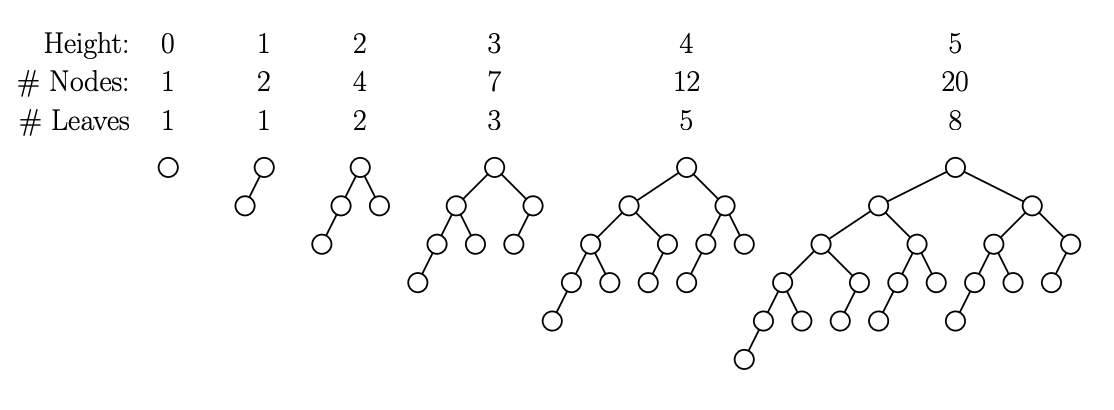
\includegraphics[width=\textwidth]{FibTreeMinNodes}
  Rotations are used to main tree's balance by modifying relation between two nodes but preserving the tree's inorder properties 
  \begin{lstlisting}
    BinaryNode rotateRight(BinaryNode p) {
      BinaryNode q = p.left;
      p.left = q.right;
      q.right = p;
      return q;   // q is now root
    }
    Binary Node rotateLeft(Binary Node p) {
      BinaryNode q = p.right;
      p.right = q.left;
      q.left = p;
      return q;   // q is now root
    }
  \end{lstlisting}
  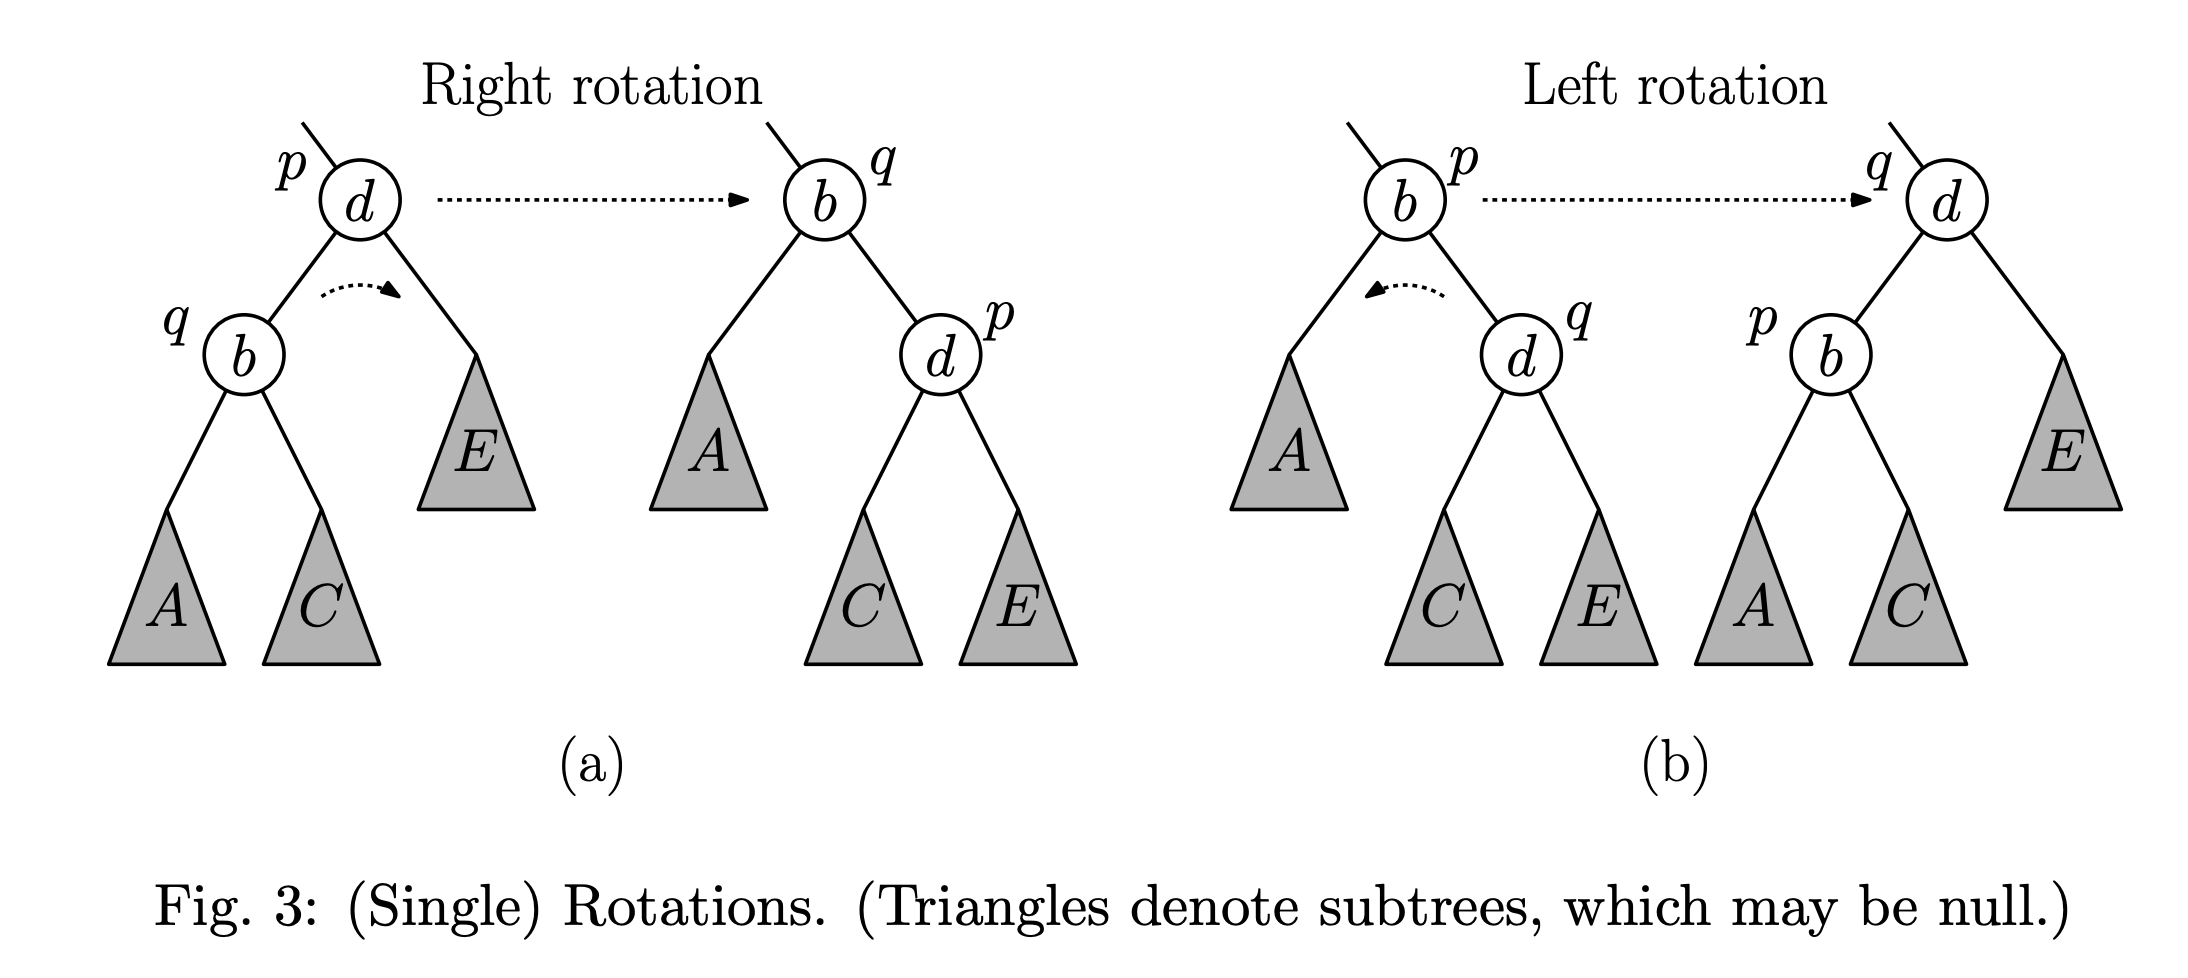
\includegraphics[width=\textwidth]{FibTreeRotation}
  Single rotations work when the imbalance occurs on the outer edges of the tree. Need to use double rotations LR or RL to balance inner trees \\
  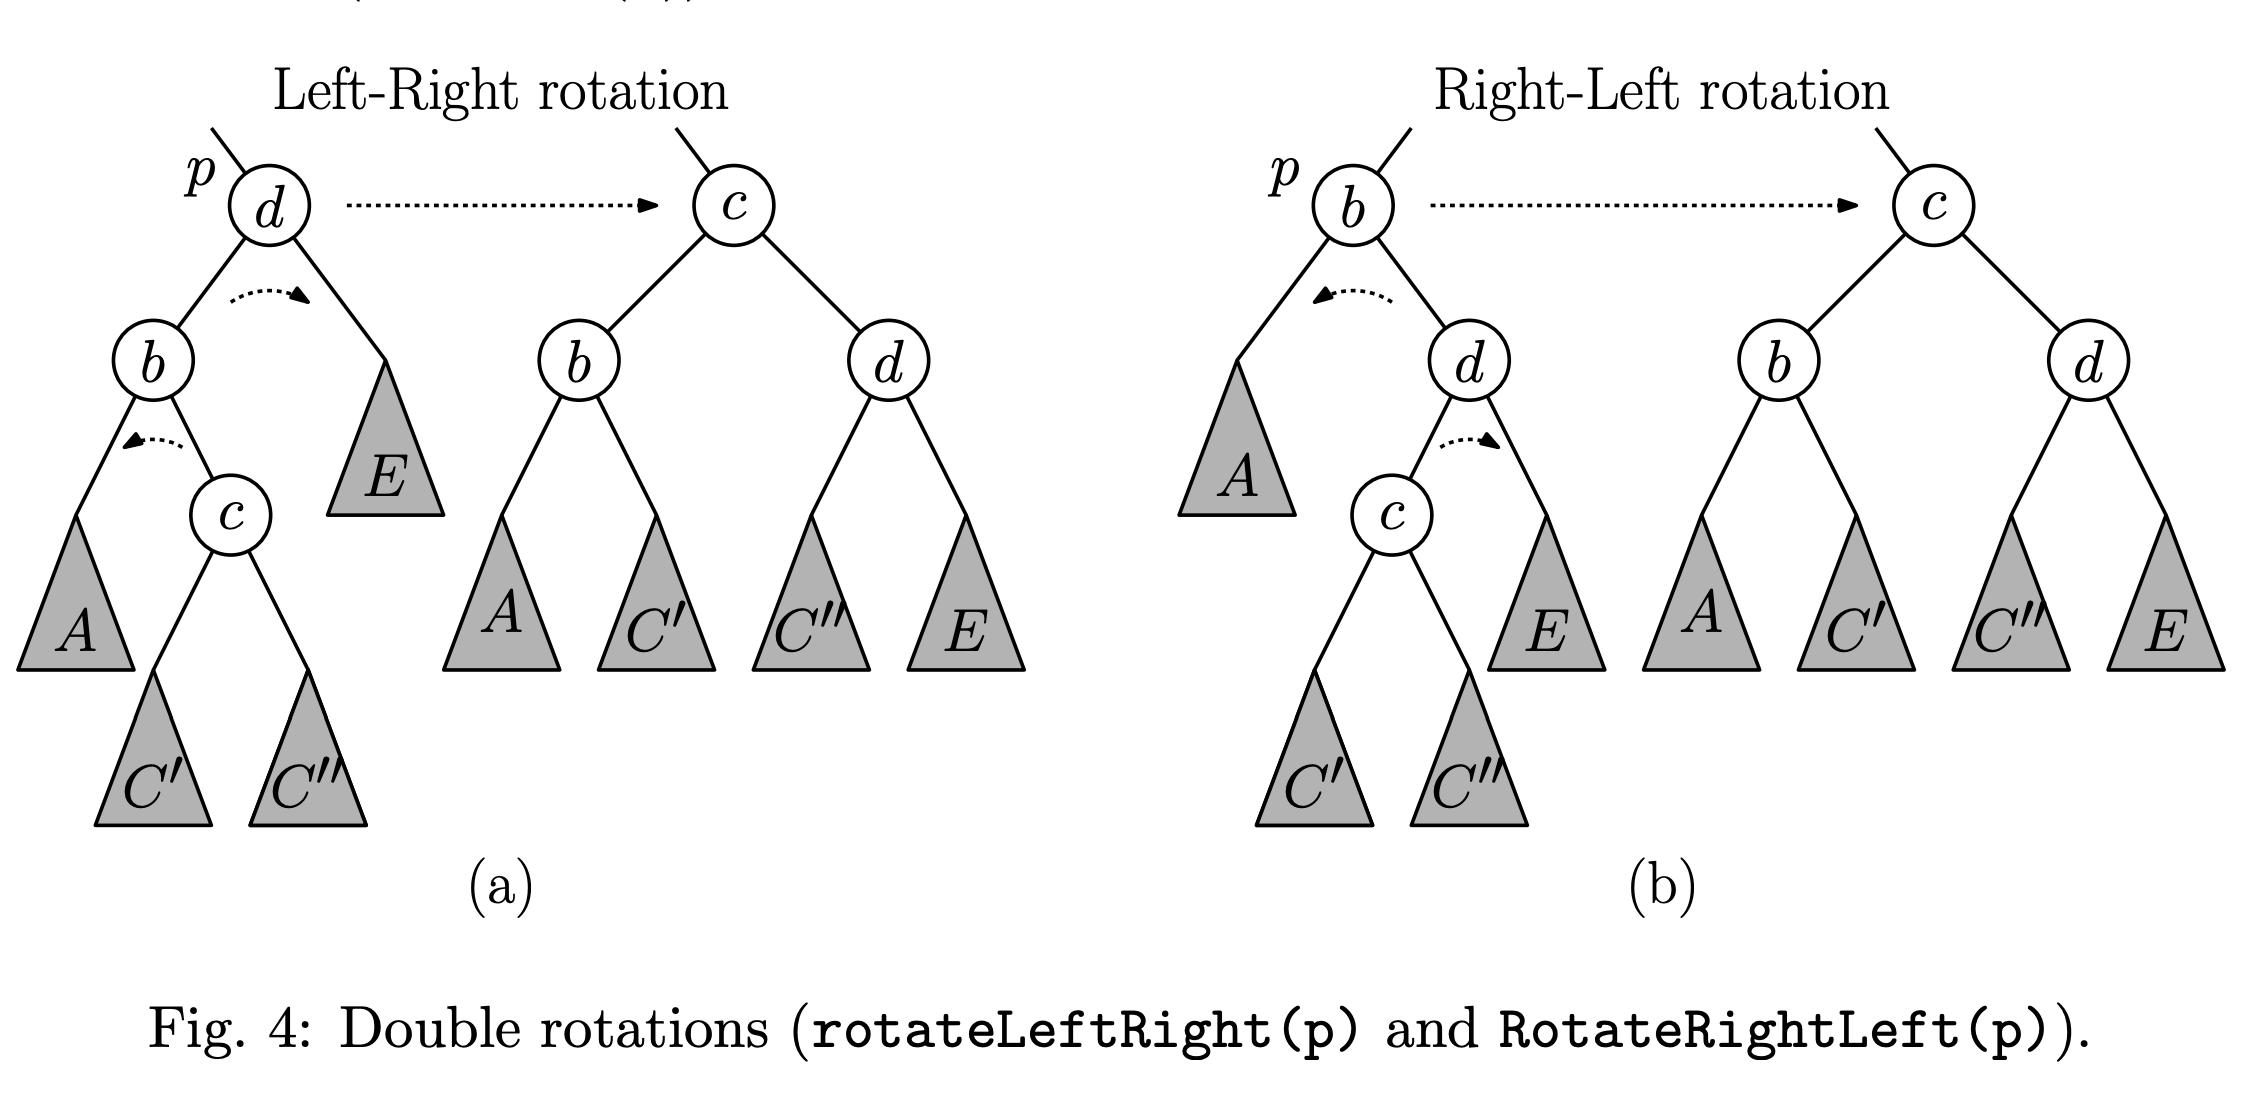
\includegraphics[width=\textwidth]{FibTreeDoubleRotation}
  Insertion works similar to BST except we update the heights of subtrees and apply rotations to maintain height \\
  When insertion occurs balance factors of ancestors is altered by $\pm$1\\
  If a node has a balance factor that violates Balance Property:
  \begin{itemize}[noitemsep]
  \item Left-Left substree too deep then rotate right 
  \item Right-Right subtree too deep then rotate left
  \item Left-Right subtree too deep then rotate left-right
  \item Right-Left subtree too deep then rotate right-left
  \end{itemize}
  \newpage
  \begin{lstlisting}
    int height(AvlNode p) return p == null ? -1 : p.height;
    void updateHeight(AvlNode p) p.height = 1 + max(height(p.left), height(p.right));
    int balanceFactor(AvlNode P) return height(p.right) - height(p.left);
    AvlNode rotateRight(AvlNode p) {
      AvlNode q = p.left;
      p.left = q.right;   // swap inner child
      q.right = p;        // bring q above p
      updateHeight(p);
      updateHeight(q);
      return q;           // q replaces p
    }
    AvlNode rotateLeft(AvlNode p) {... symmetrical to rotateRight ...}
    AvlNode rotateLeftRight(AvlNode p) {
      p.left = rotateLeft(p.left);
      return rotateRight(p);
    }
    AvlNode rotateRightLeft(AvlNode p) {... symmetrical to rotateLeftRight ...}
    AvlNode insert(Key x, Value v, AvlNode p) {
      if (p == null) p = newAvlNode(x, v, null, null);
      else if (x < p .key) p.left = insert(x, v, p.left);
      else if (x > p.key) p.right = insert(x, v, p.right);
      else throw DuplicateKeyException;
      return rebalance(p);
    }
    AvlNode rebalance(AvlNode p) {
      if (p == null) return p;
      if (balanceFactor(p) < -1) {
        if (height(p.left.left) >= height(p.left.right)) {//left-left heavy
          p = rotateRight(p);
        } else {                                          //left-right heavy
          p = rotateLeftRight(p);
        }
      }
      else if (balanceFactor(p) > 1) {
        if(height(p.right.right) >= height(p.right.left)) {//right-right heavy
          p = rotateLeft(p);
        } else {                                            //right-left heavy
          p = rotateRightLeft(p);
        }
      }
      updateHeight(p);
      return p;
    }
  \end{lstlisting}
  Deletion works in a similar manner in that we call normal BST delete and then rotate as necessary. However we need to call rebalance on further ancestors to check balance condition (e.g. if one of the inner subtrees is too tall, we need to call a double rotation)
  \newpage 
  \section{2-3 Trees, Red-Black Trees, AA Trees}
  \subsection{2-3 Trees}
  nodes can either be 2-node (normal binary tree) or 3-node (2 keys b,d and 3 branches A, C, E where A $<$ b $<$ X $<$ d $<$ E)\\
  All leaves are on the same level \\
  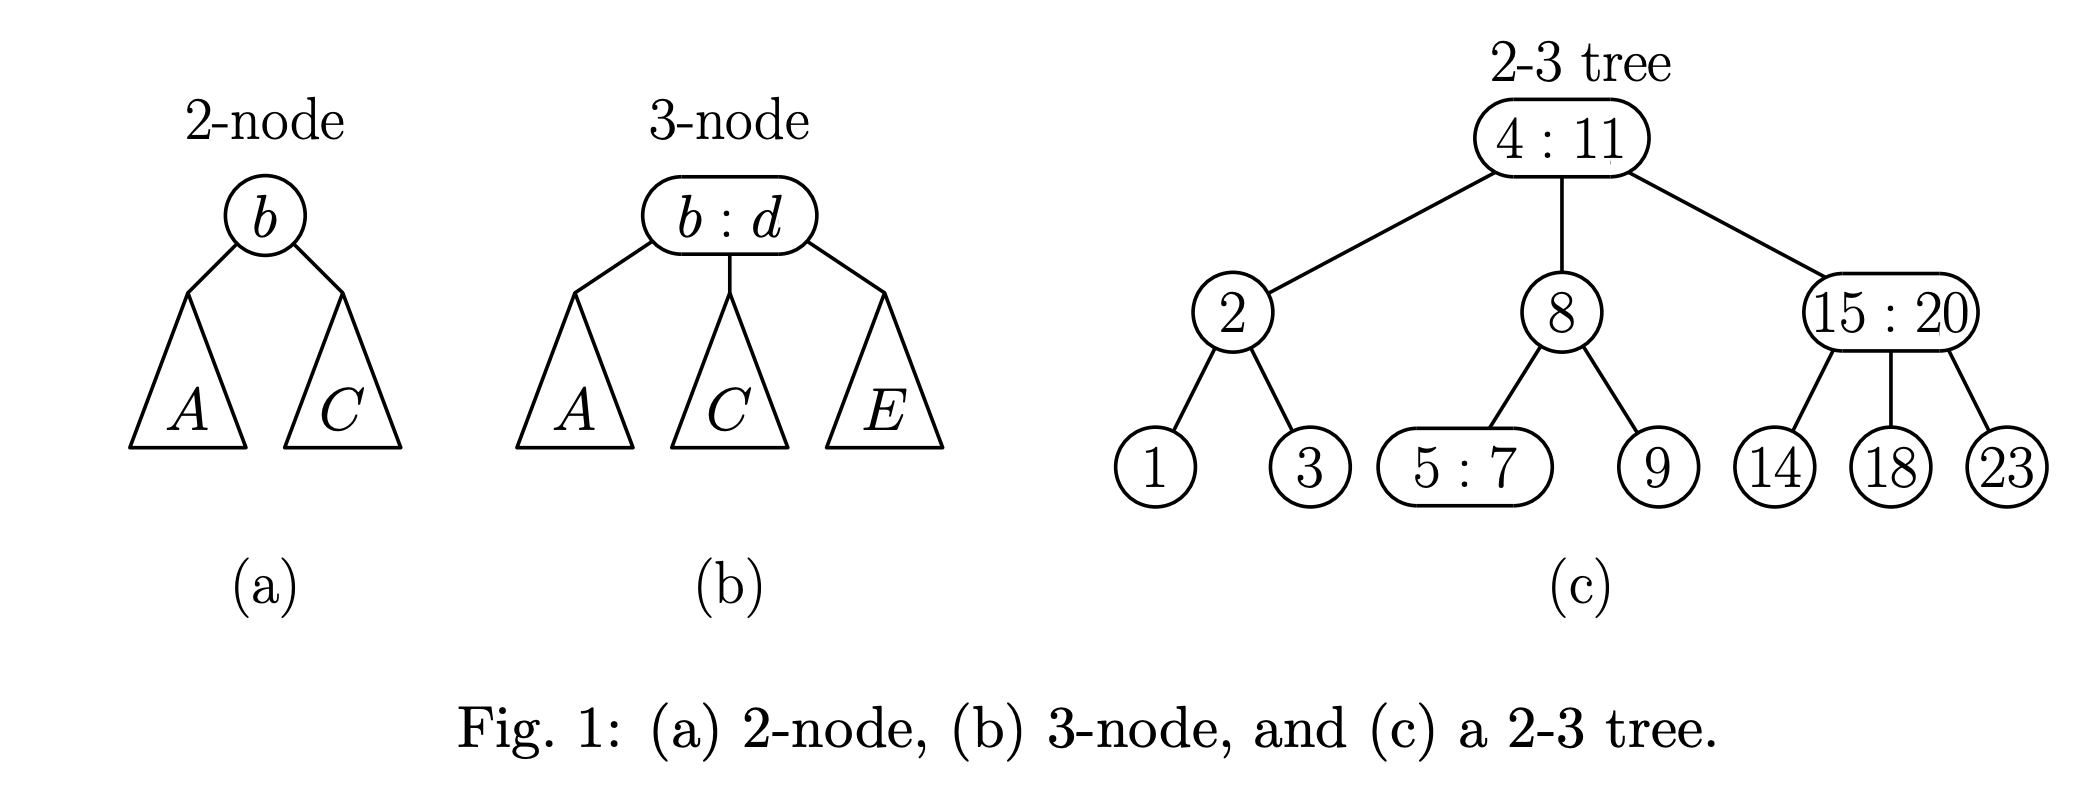
\includegraphics[width=\textwidth]{2-3Tree}
  Recursively defined as:
  \begin{itemize}[noitemsep]
  \item empty (null)
  \item root is 2-node and has two 2-3 subtrees of equal height
  \item root is 3-node and has three 2-3 subtrees of equal height
  \end{itemize}
  Sparsest 2-3 tree is a complete binary tree \\ \\
  Find: recursive descent but when 3-node is reached, compare x with both keys to find which branch to go to\\ \\
  Insertion: search for key and and insert like in a normal tree.
  \begin{itemize}[noitemsep]
  \item if parent is a 2-node, now it is a 3-node with a null subtree
  \item if parent is 3 node then it becomes 4-node and we have to fix it by splitting the 4-node into two 2-nodes and prop the middle term up for recursion and will continue to recurse up until it reaches the root \\
  \end{itemize}
  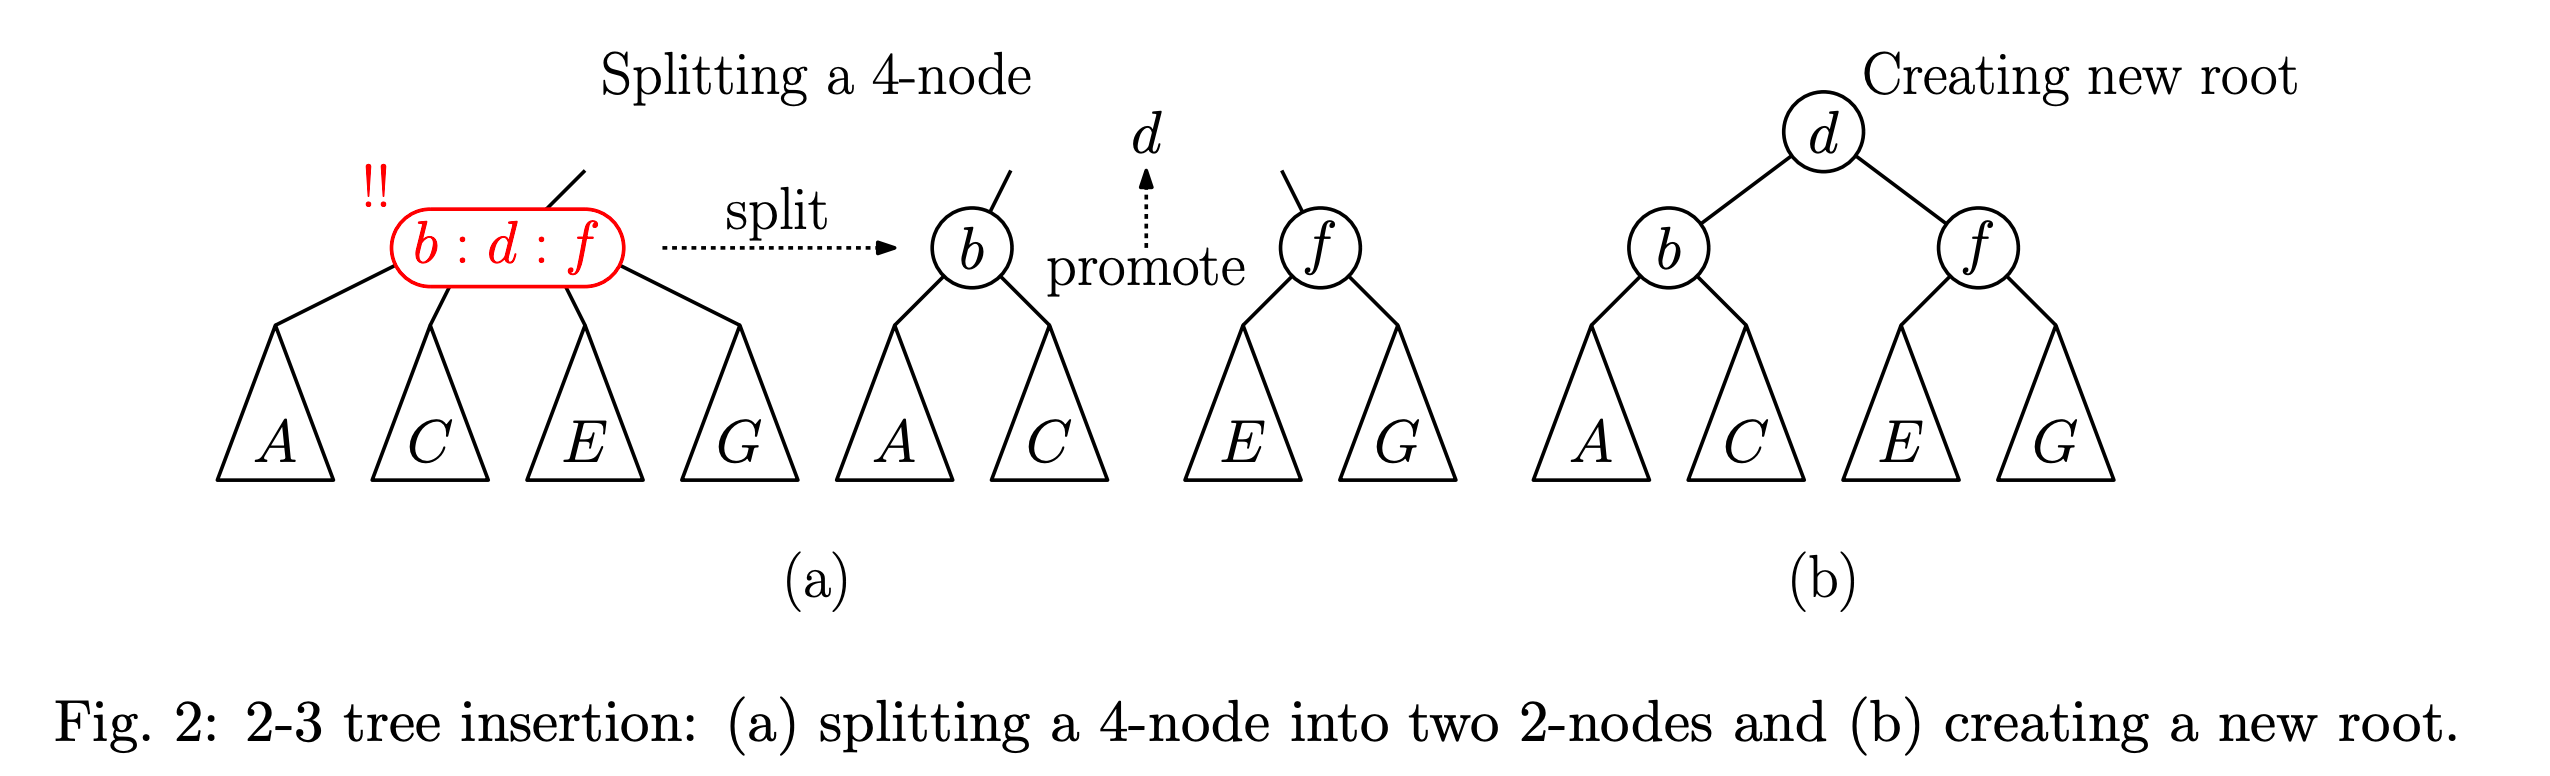
\includegraphics[width=\textwidth]{2-3TreeInsert}
  Deletion: find and replace target with inorder successor and then delete the leaf
  \begin{itemize}[noitemsep]
  \item If parent of leaf is a 3-node then parent becomes a 2-node and done
  \item If parent is a 2-node then it becomes a 1-node (0 keys, 1 subtree) so we can do
    \begin{itemize}[noitemsep]
      \item Adoption: if sibling is a 3-node then adopt a key and a subtree so we have two 2-nodes
      \item Merge: merge 1-node and 2-node and take a key from parent then recurse up. If root is reached, remove it and make a child the root
    \end{itemize}
  \end{itemize}
  \subsection{Red-Black Trees}
  Take a 3-node and create a 2-node combo by using d, C, E as the right subtree and b, A for left subtree \\
  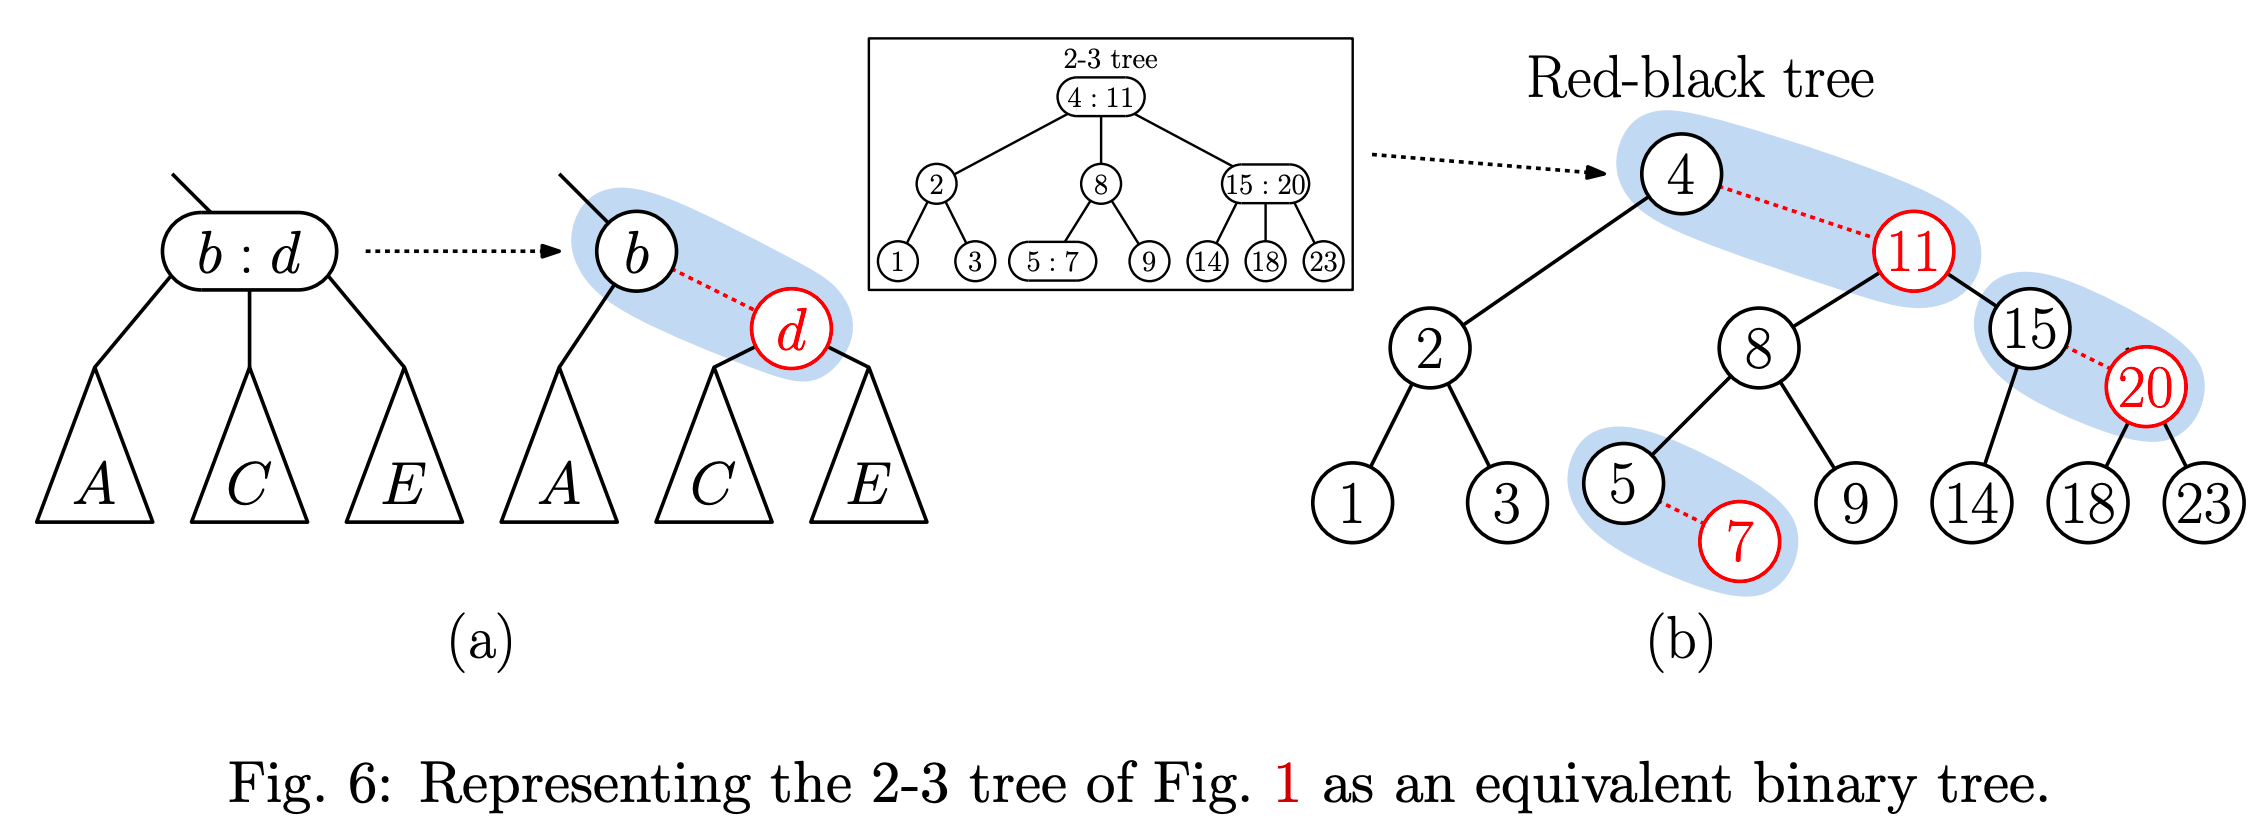
\includegraphics[width=\textwidth]{RBTree}
  Created right subnode is red and all other nodes black, creating a binary search tree\\
  Null pointers are labeled black and if a node is red, then both its children are black \\
  Every path from a given node to any of its null descendants contains the same number of black nodes\\
  O(logn) height \\
  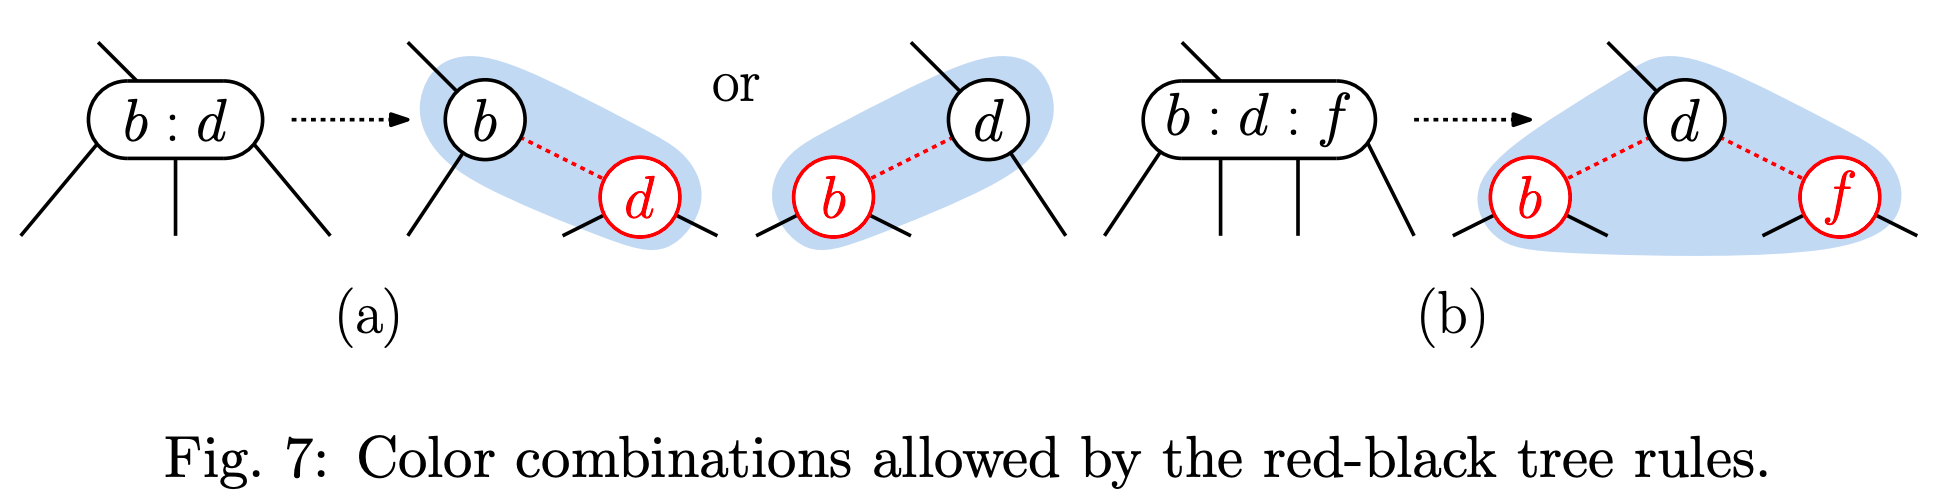
\includegraphics[width=\textwidth]{2-3ToRBTree}
  Every 2-3 tree corresponds to a red-black tree but converse is not true
  \begin{itemize}[noitemsep]
  \item Issue with RB tree doesn't distinguish between L and R children so 3-node can be encoded in 2 different ways
  \item Also can't convert a node with 2 red children to 2-3 tree which ends up being a 4-node
  \end{itemize}
  \newpage
  \subsection{AA Trees}
  Simplified RB tree where red nodes can only appear as right children of black nodes allowing conversion between 2-3 tree and RB trees \\
  Edge between red node and the black parent is called a red edge \\
  Implementation of AA trees also uses a sentinel node nil where every null pointer is replaced with a pointer to nil
  \begin{itemize}[noitemsep]
  \item In this case, nil.left == nil.right == nil so we don't have to keep doing null checks
  \end{itemize}
  Implementation of AA doesn't store colors. Instead stores level of associated node in 2-3 tree
  \begin{itemize}[noitemsep]
  \item nil = level 0
  \item If black, p.level = q.level (child) + 1
  \item If red, then same level as parent. Now can easily test if node is read by comparing with parent level
  \end{itemize}
  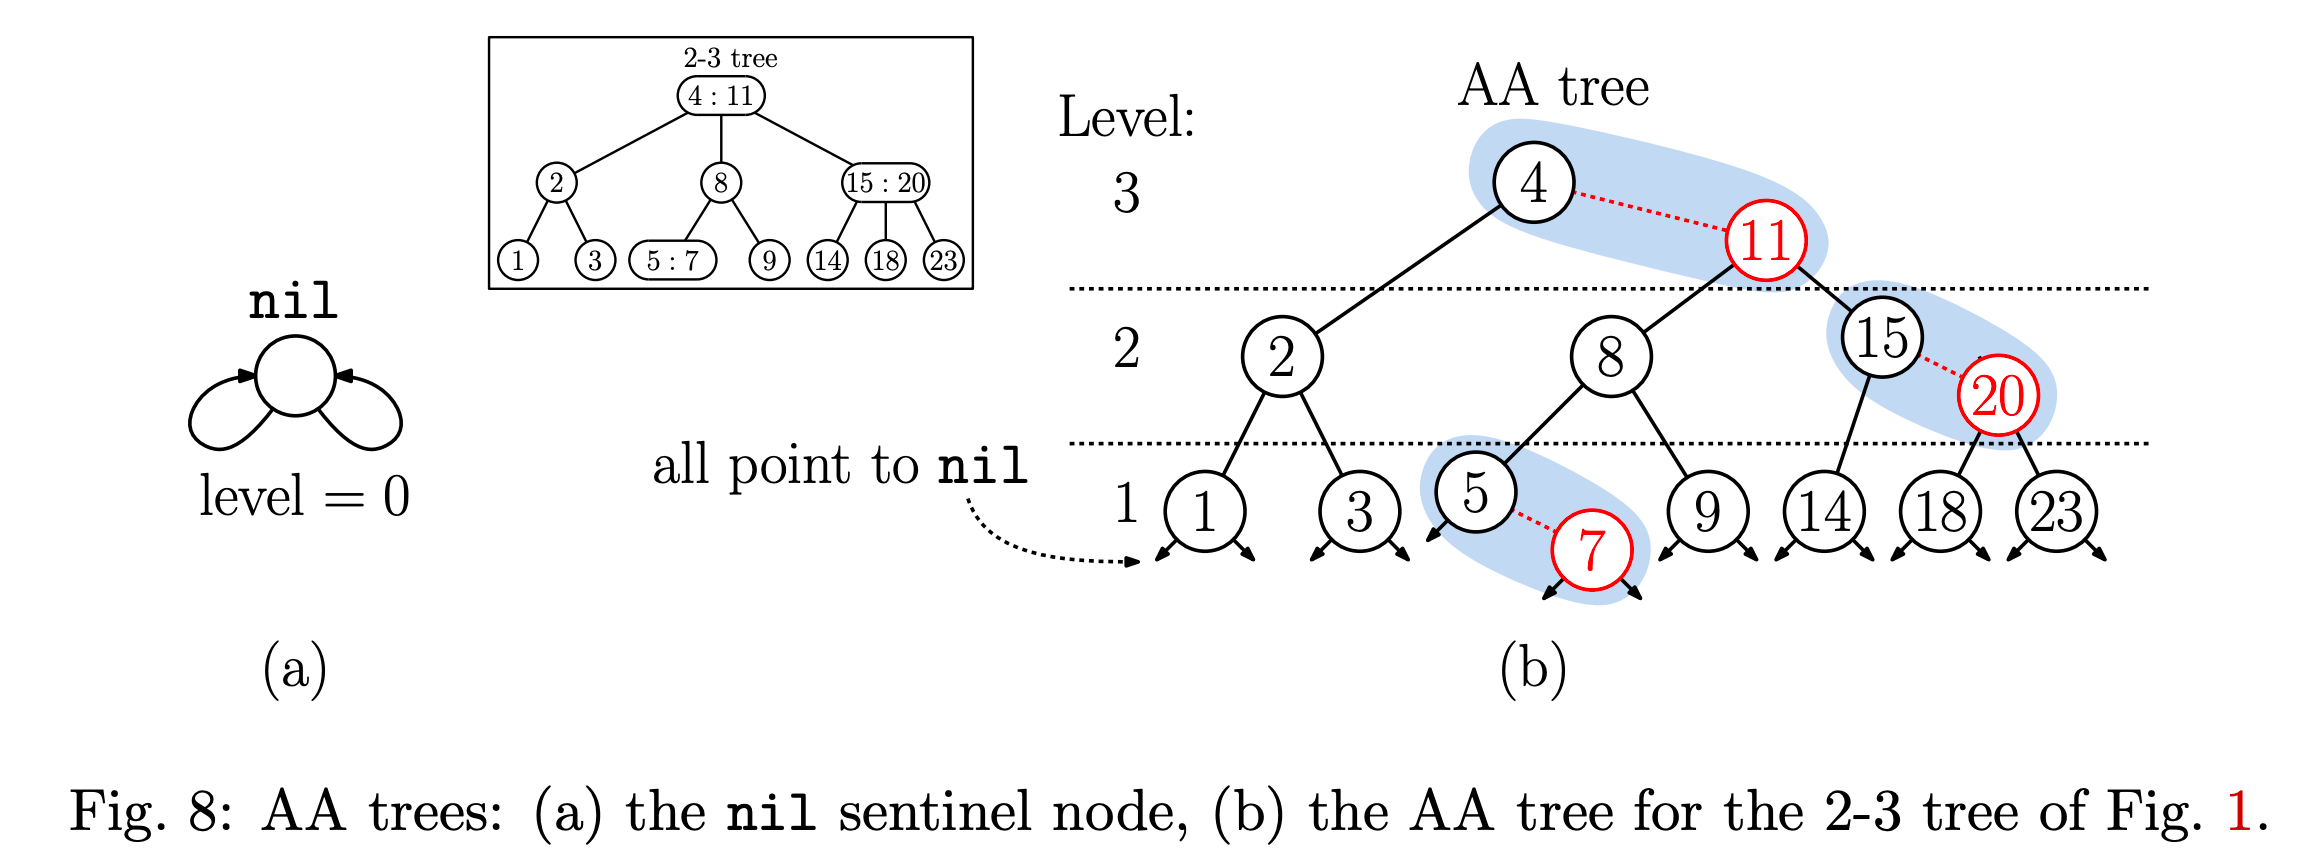
\includegraphics[width=\textwidth]{AATree}
  Find method works exactly the same as it does for BST \\ \\
  Insertion and Deletion require skew(p) and split(p)
  \begin{itemize}[noitemsep]
  \item skew(p) if p is black and has a red left child, rotate right
  \item split(p) if p is black and has right-right chain, do a left rotation \& promote first red child to next level
  \end{itemize}
  \begin{lstlisting}
    AANode skew(AANode p) {   
      if (p.left.level == p.level) {  // red node to our left?
        AANode q = p.left;            // do right rotation at p
        p.left = q.right;
        q.right = p;
        return q;
      }
      else return p;
    }
    AANode split(AANode p) {
      if (p.right.right.level == p.level) {   //right-right red chain?
        AANode q = p.right;                   // do left rotation at p
        p.right = q.left;
        q.left = p;
        q.level += 1;                         // promote q to higher level
        return q;
      }
      else return p;
    }
  \end{lstlisting}
  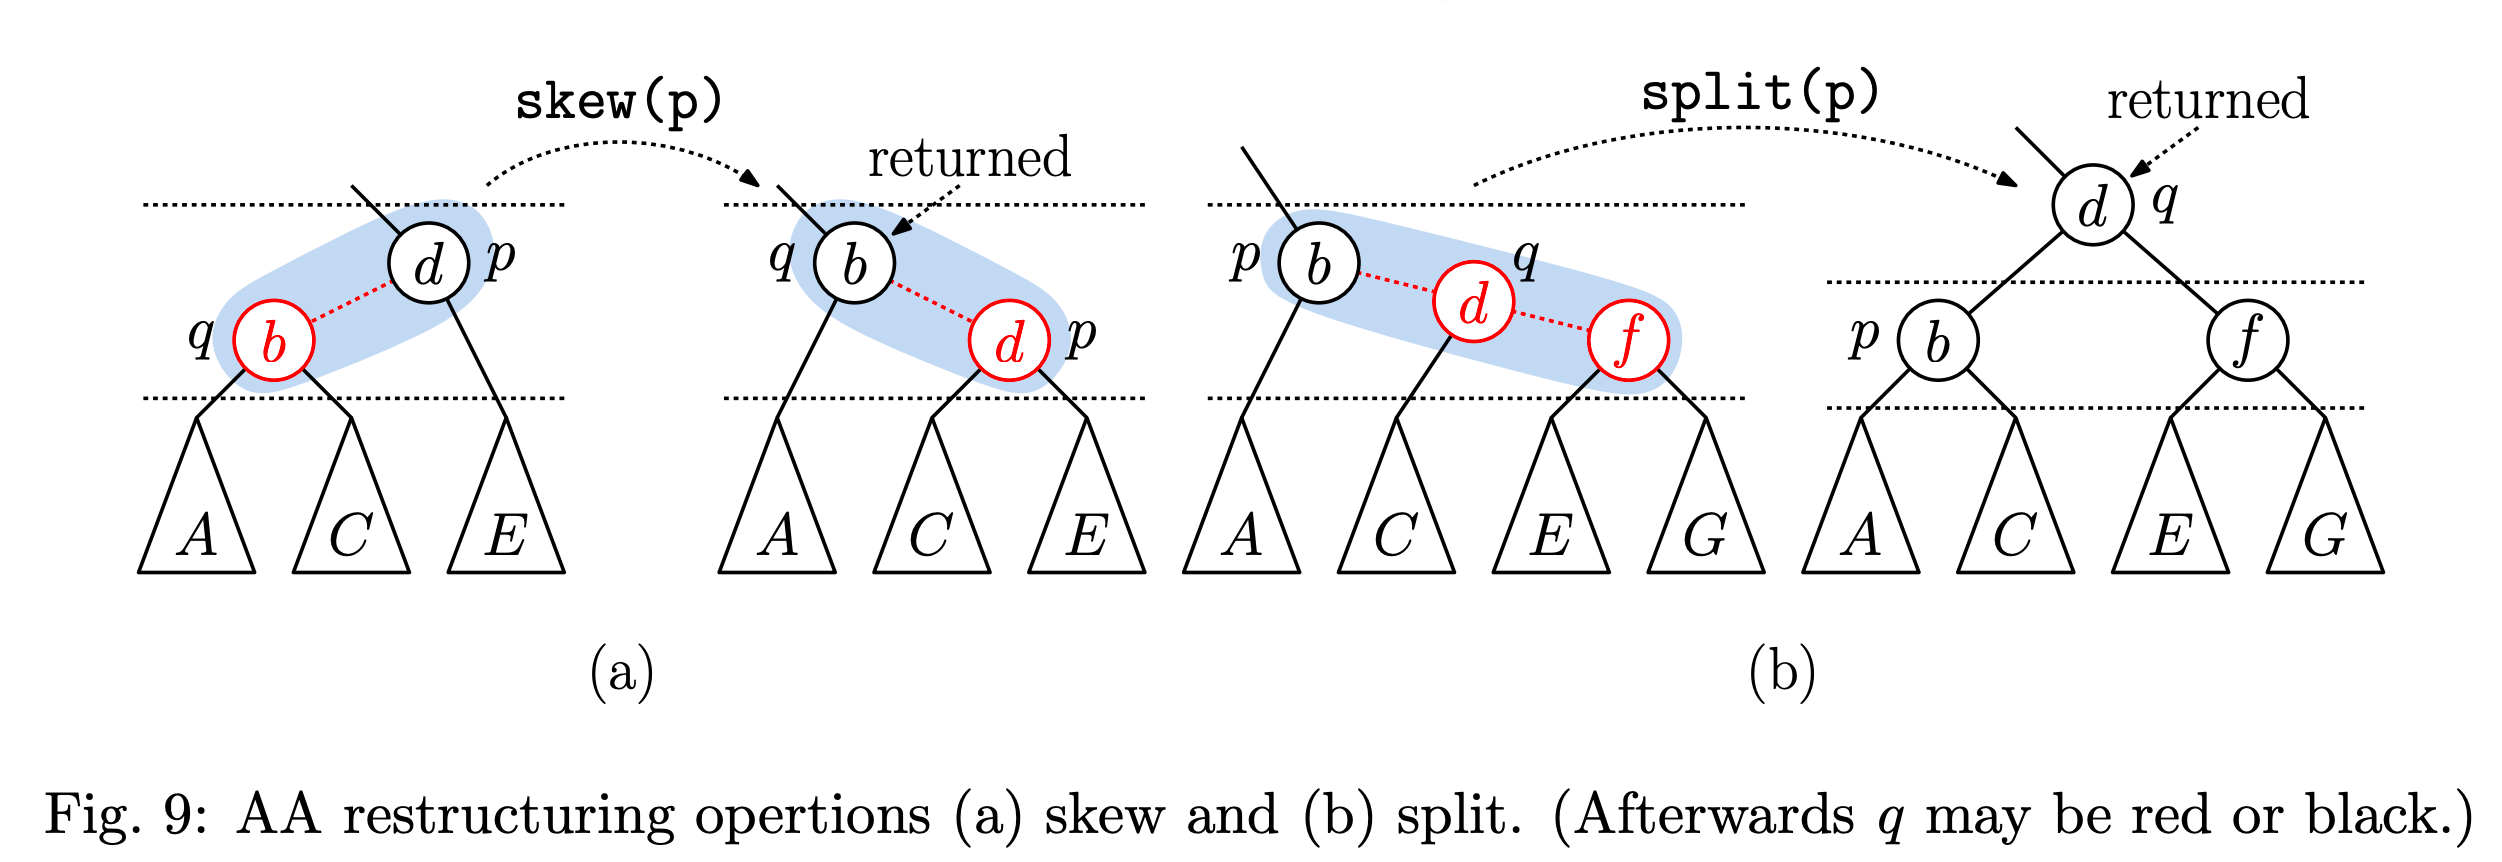
\includegraphics[width=\textwidth]{AASkewSplit}
  Insertion: insert node like in BST except treat it as a red node then work back up tree restructuring as we go. 
  \begin{itemize}[noitemsep]
  \item If red node inserted as left child then perform skew(p) on parent
  \item If red node inserted as right child of red node, call split(p) on grandparent and then recurse up to fix any issues
  \end{itemize}
  \begin{lstlisting}
    AANode insert(Key x, Value v, AANode p) {
      if (p == nil) p = new AANode(x, v, 1, nil, nil)       //fell out so create new leaf
      else if (x < p.key) p.left = insert(x, v, p.left);
      else if (x > p.key) p .right = insert(x, v, p.right);
      else throw DuplicateKeyException;
      return split(skew(p));        //restructure (if not needed split and skew return unmodified tree)
    }
  \end{lstlisting}
  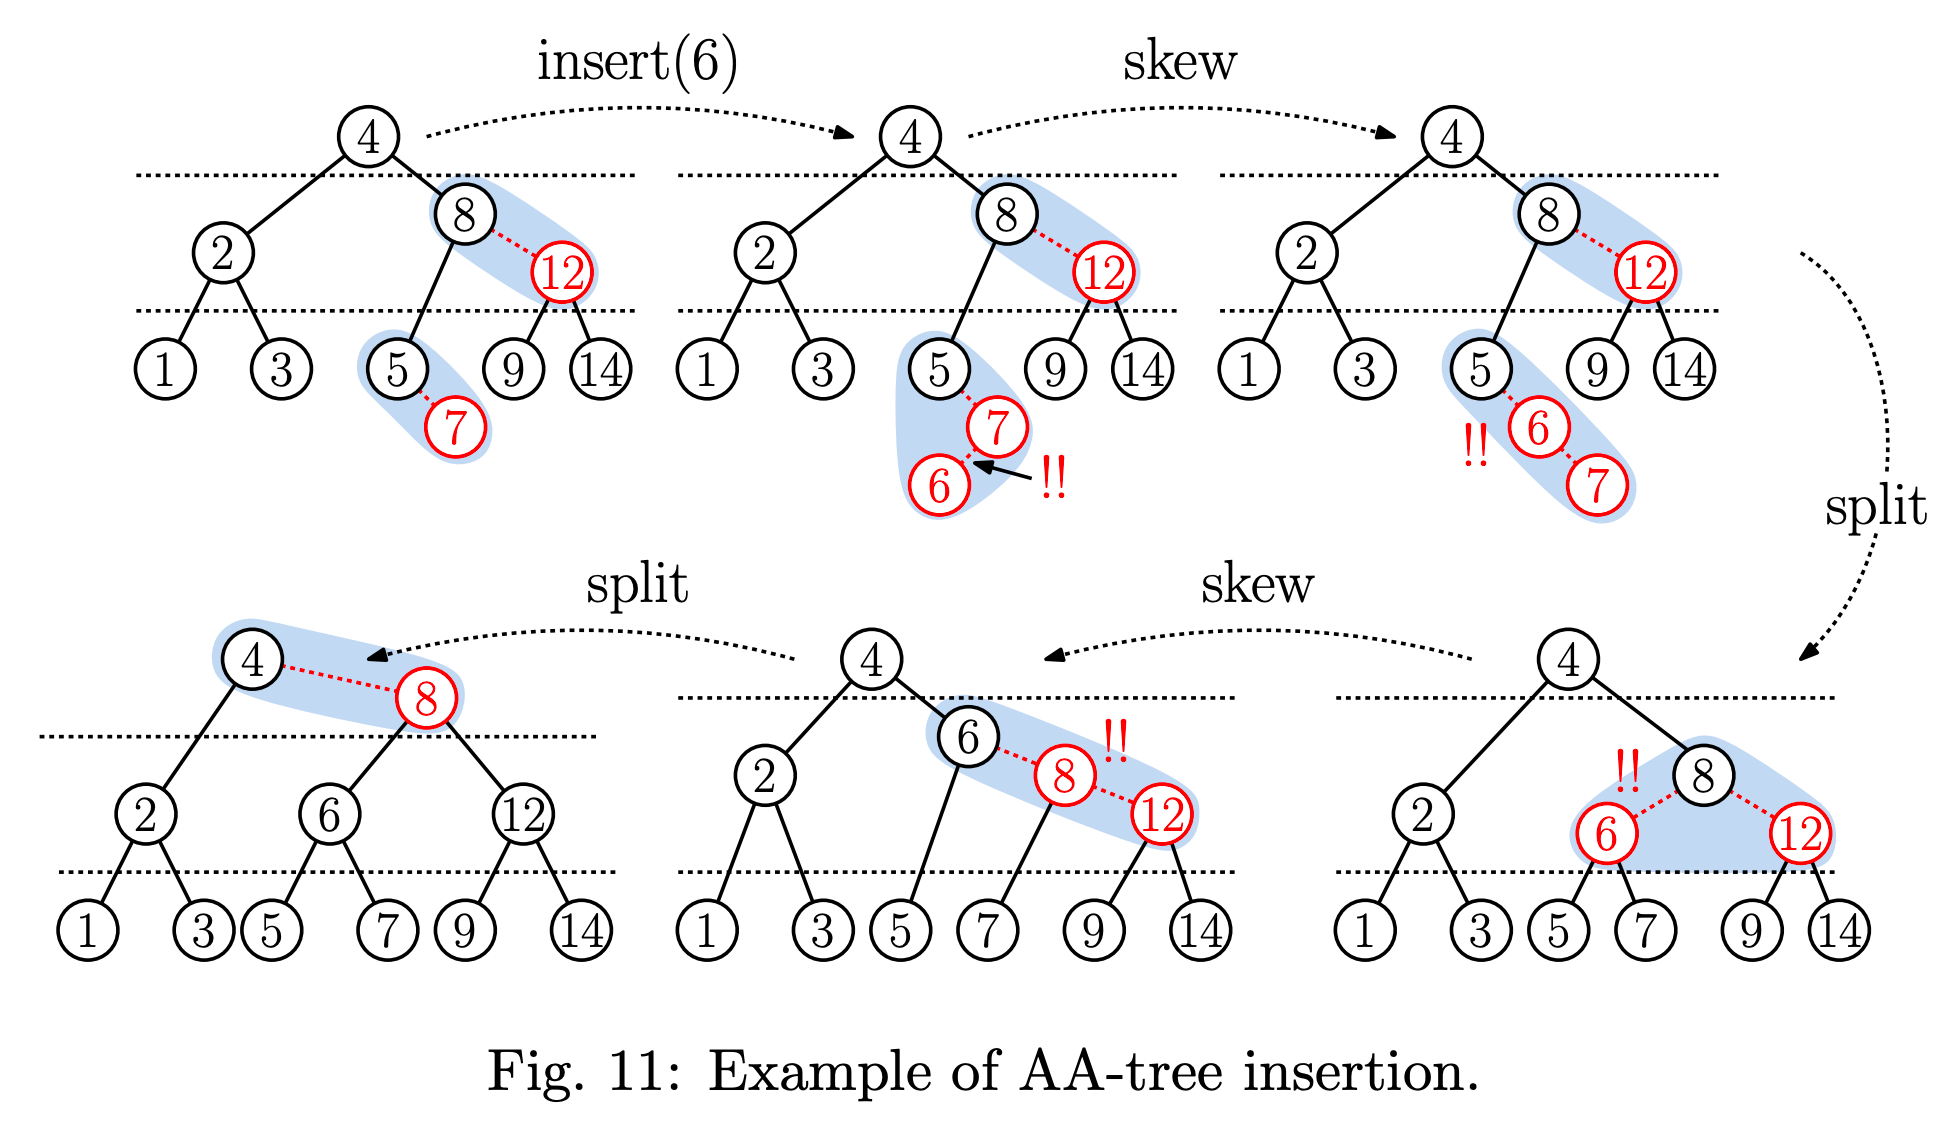
\includegraphics[width=\textwidth]{InsertionAATree}
  Deletion: Replace target node with inorder successor then delete leaf and retrace search path to restructure tree
  \begin{itemize}[noitemsep]
  \item use updateLevel(p) helper to update level of node p based on children
    \begin{itemize}[noitemsep]
      \item since every node has at least 1 black node, ideal level for any node is 1 + min of its children 
      \item if p is updated and right child is red then we need to update p.right.level = p.level
    \end{itemize}
  \end{itemize}
  \begin{lstlisting}
    AANode updateLevel(AANode p) {
      int idealLevel = 1 + min(p.left.level, p.right.level);
      if (p.level > idealLevel) {
        p.level = idealLevel;
        if(p.right.level > idealLevel) p.right.level = idealLevel;  //is right child a red node?
      }
    } 
  \end{lstlisting}
  Use fixupAfterDelete(p) to make sure any red children are on the right
  \begin{itemize}[noitemsep]
  \item May need to call up to 3 skew operations (p, p.right, p.right.right) and then 2 splits (p and its right-right grandchild). The example below shows how there might be a 2 level gap between a parent and a child, which could end up necessitating 3 skew operations which then require 2 splits to fix
  \end{itemize}
  \begin{lstlisting}
    AANode fixupAfterDelete(AANode p) {
      p = updateLevel(p);
      p = skew(p);
      p.right = skew(p.right);
      p.right.right = skew(p.right.right);
      p = split(p);
      p.right = split(p.right);
      return p;
    }
  \end{lstlisting}
  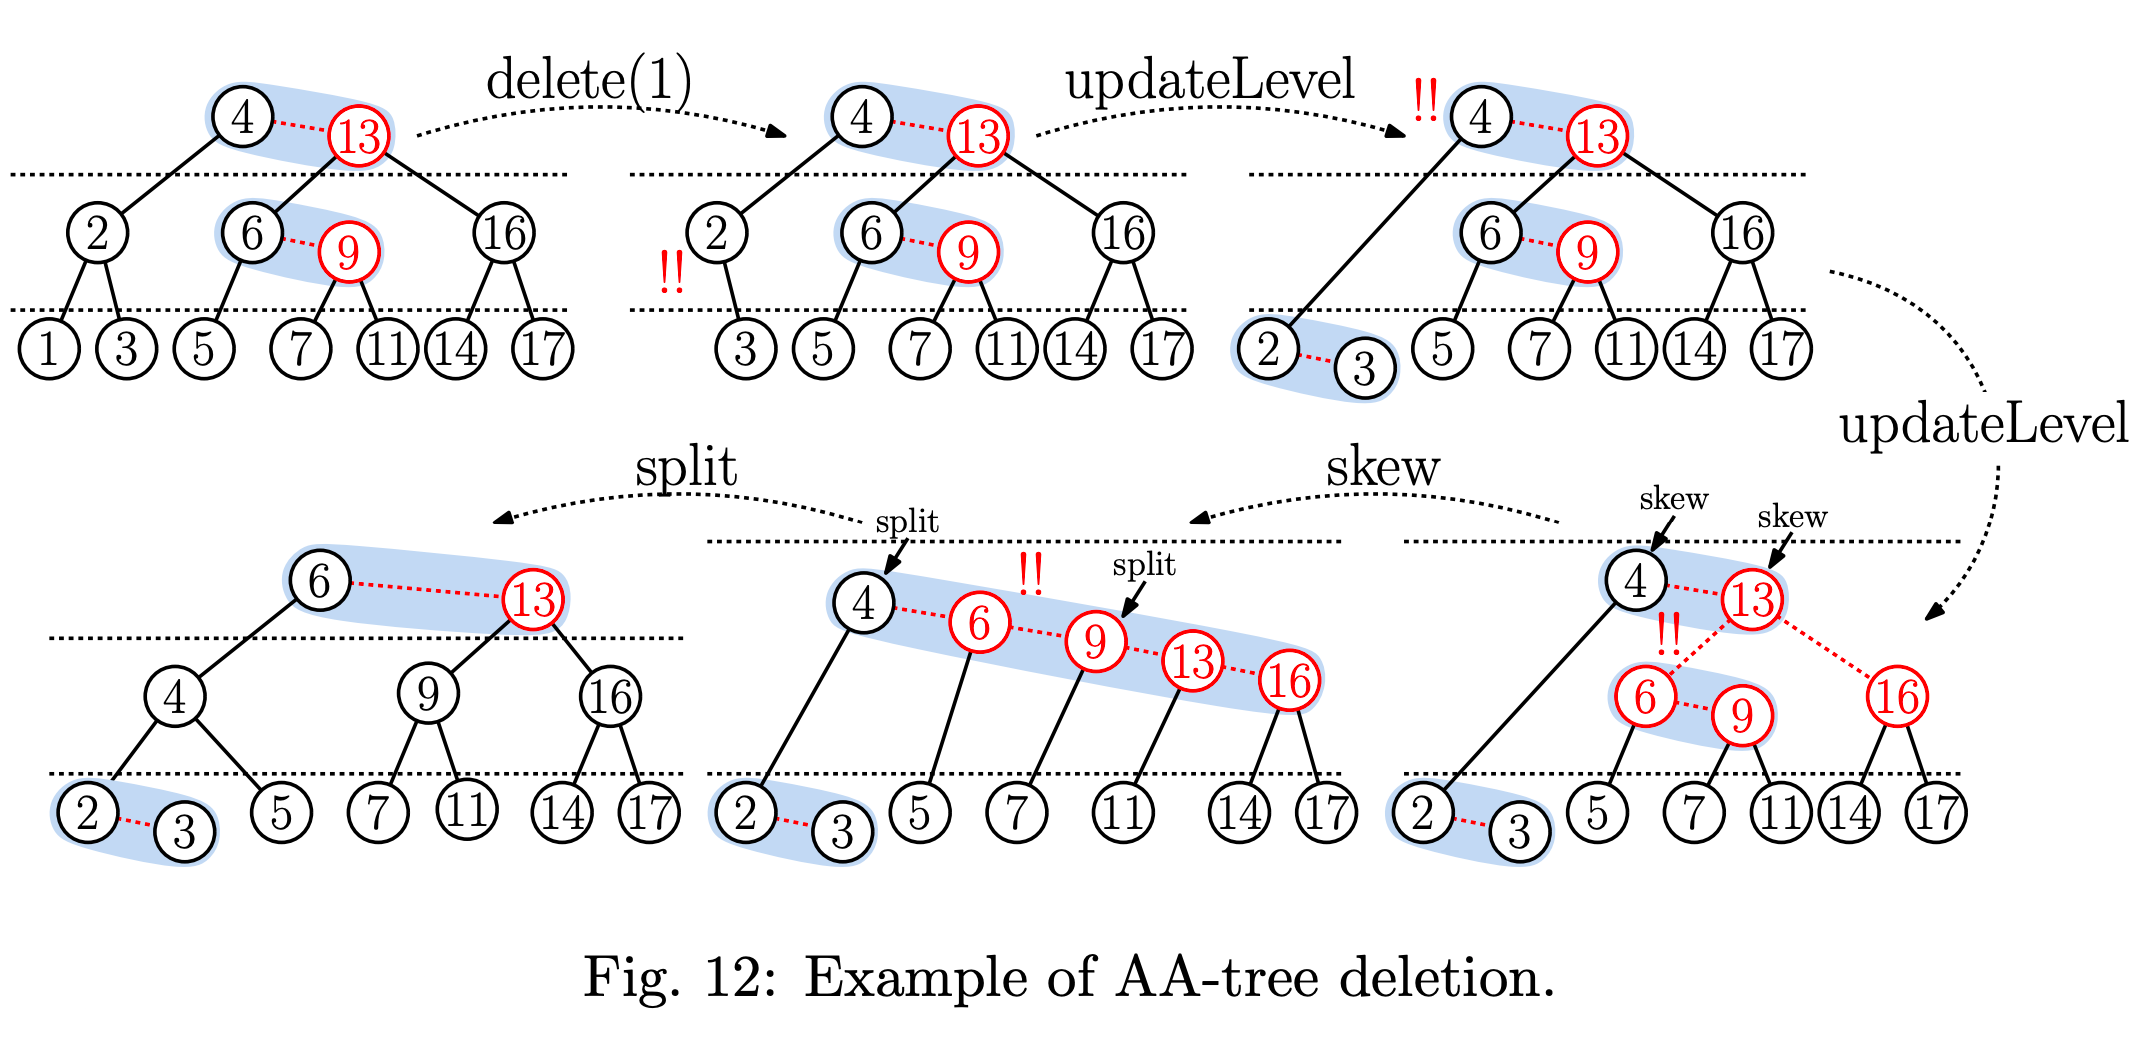
\includegraphics[width=\textwidth]{DeletionAATree}
  \newpage
  \begin{lstlisting}
    AANode delete(Key x, AANode p) {
      if (p == nil) throw KeyNotFoundException;
      else {
        if (x < p.key) p.left = delete(x, p.left);
        else if (x > p.key) p.right = delete(x, p.right);
        else {
          if (p.left == nil && p.right == nil) return nil;
          else if (p.left == nil) {           //no left child
            AANode r = inOrderSuccessor(p);
            p.copyContentsFrom(r);
            p.right = delete(r.key, p.right);
          } else {                            //no right child
            AANode r = inOrderPrdecessor(p);
            p.copyContentsFrom(r);
            p.left = delete(r.key, p.left);
          }
        }
        return fixupAfterDelete(p);
      }
    }
  \end{lstlisting}
  \newpage
  \section{Treaps and Skip Lists}
  \subsection{Treaps}
  Intuition is that if keys are inserted into BST in random order, then height will be $\approx$ O(log(n))\\ \\
  Insertion: Insert node based on key value then assign it a random priority (p.priority) and sort based on this priority by rotating the tree several times to balance it based on p.priority\\
  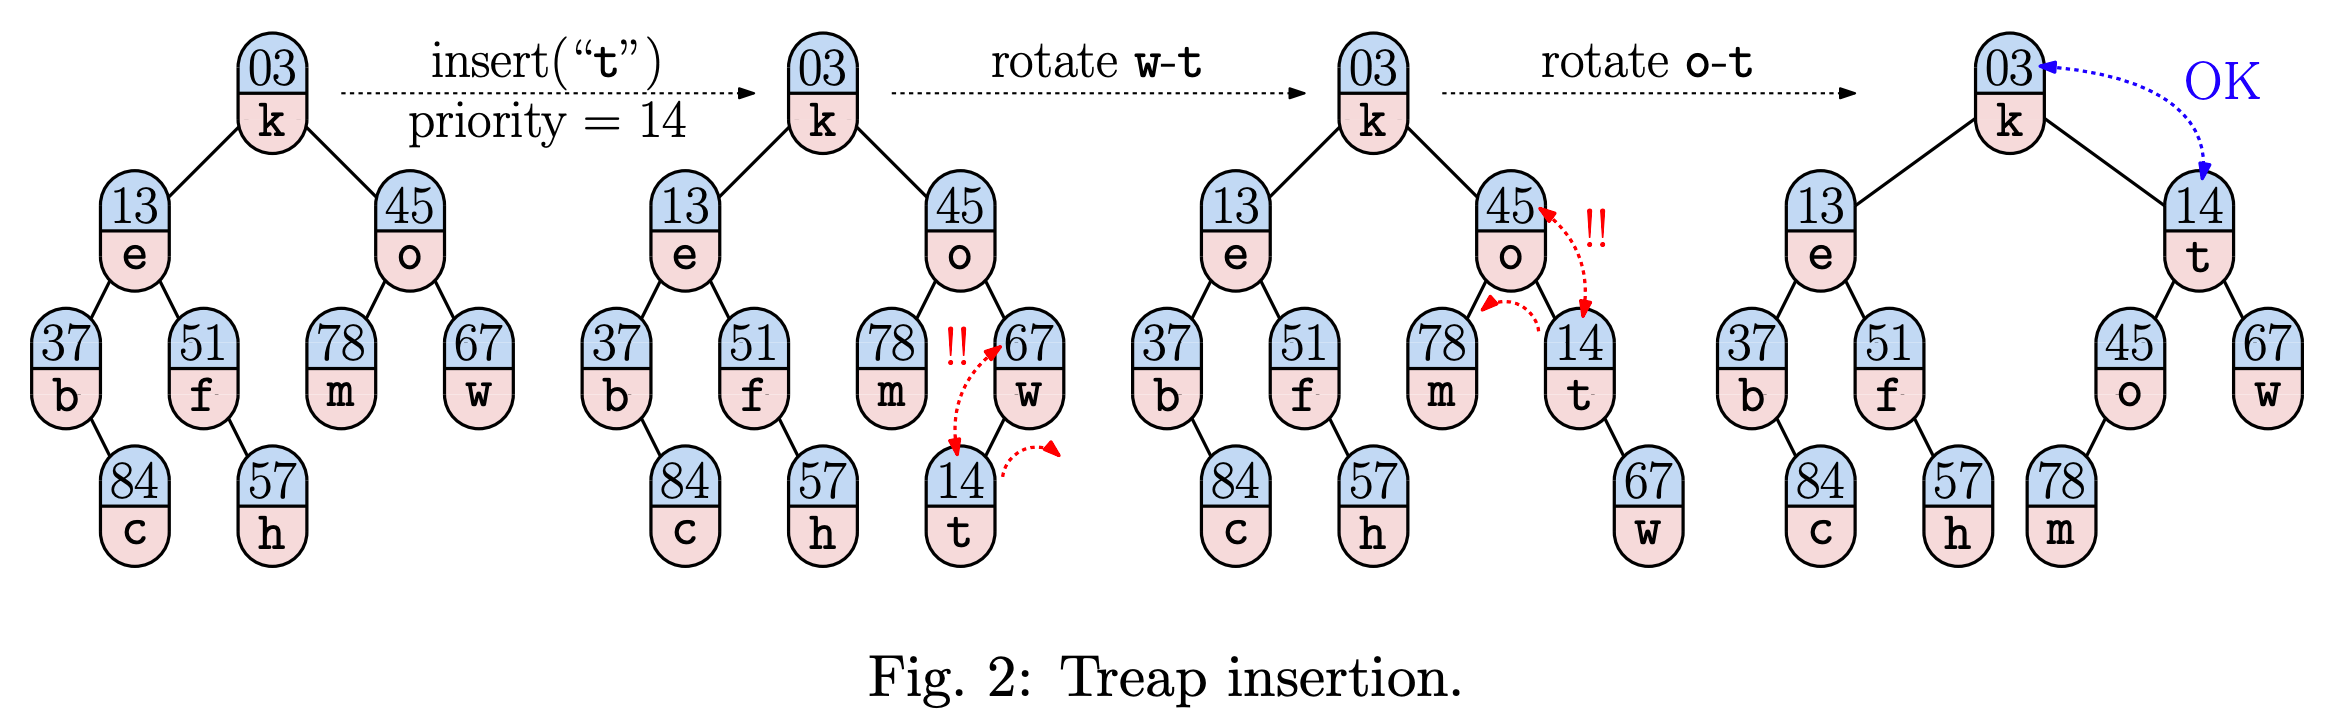
\includegraphics[width=\textwidth]{TreapInsertion}
  Deletion: 3 cases
  \begin{itemize}[noitemsep]
  \item node is leaf just remove it
  \item node has 1 child then replace node with child
  \item node has 2 children then set its priority to $\infty$ and apply rotations to sift down to leaf and remove
  \end{itemize}
  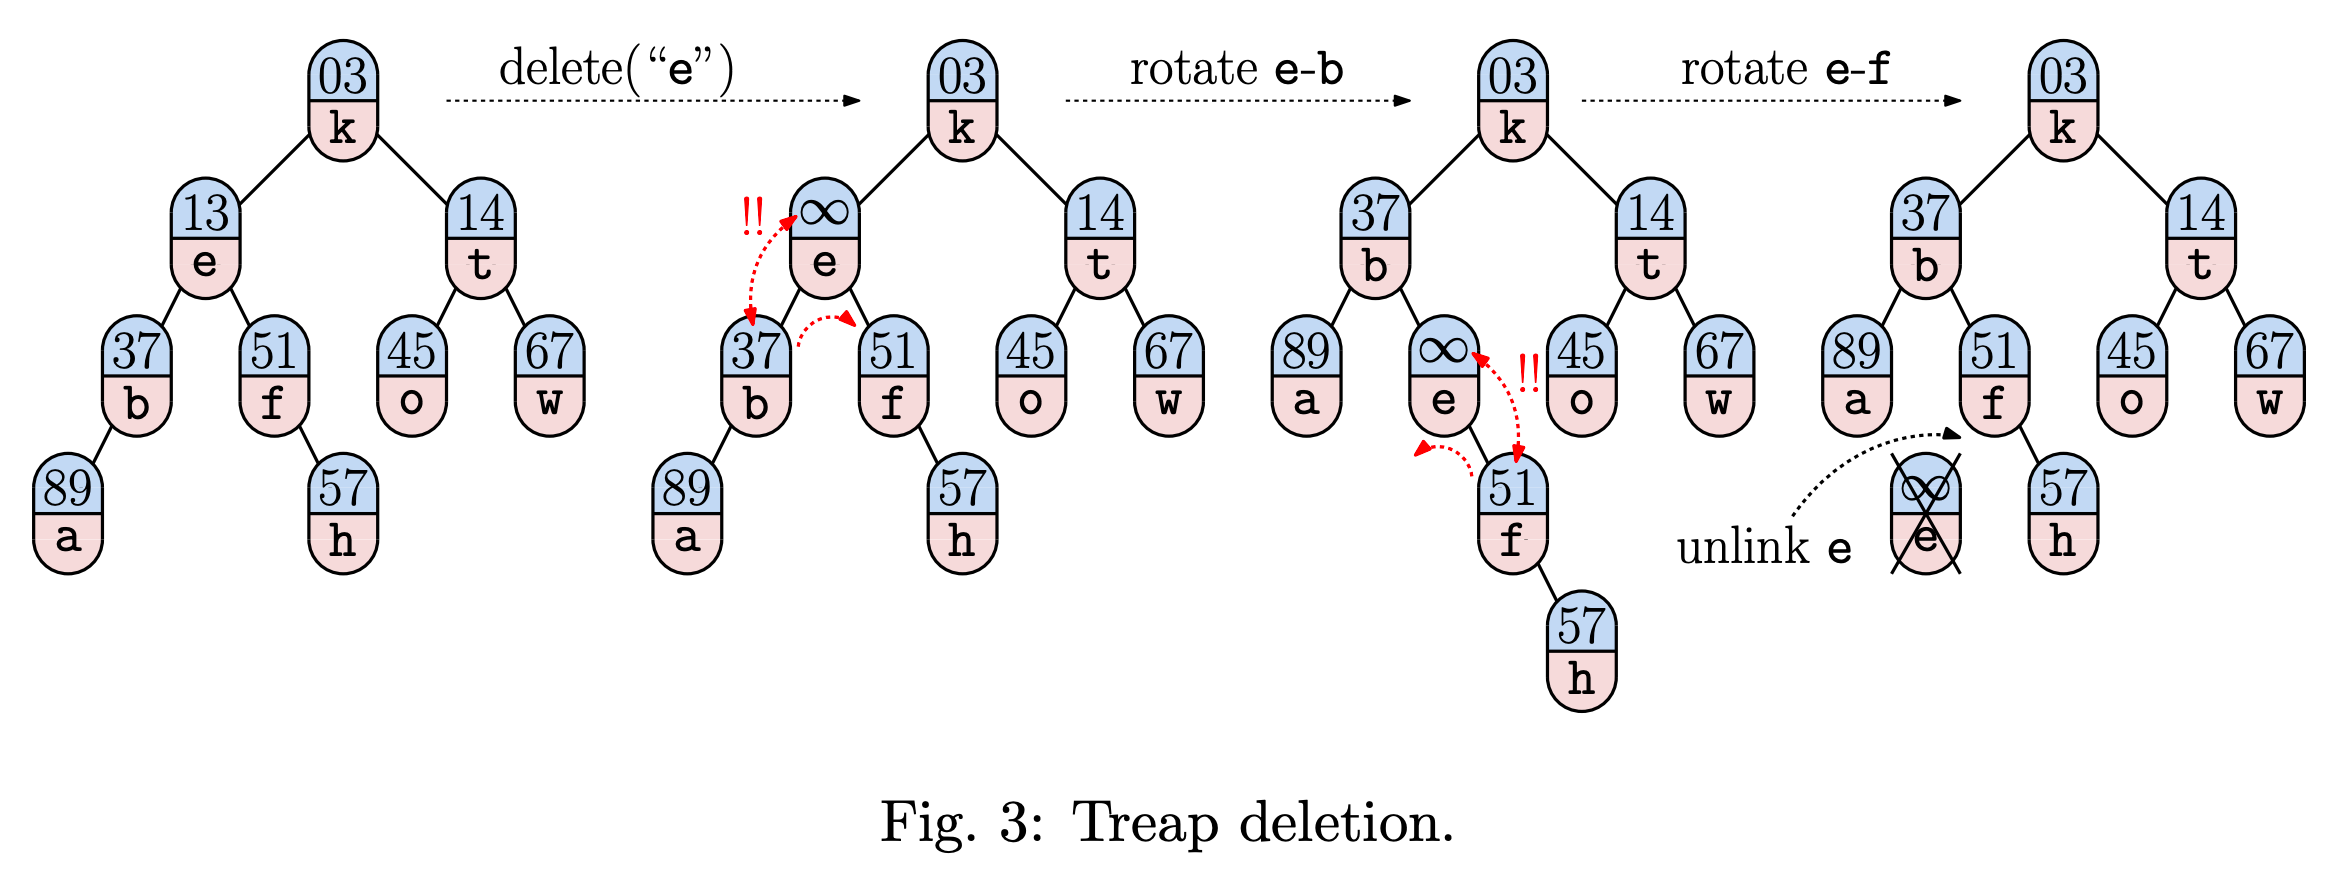
\includegraphics[width=\textwidth]{TreapDeletion}
  \newpage
  \subsection{Skip Lists}
  Intution is to skip multiple items at a time to speed up searching \\
  Skip Lists made up of multiple levels that are built from
  \begin{itemize}[noitemsep]
  \item Taking every other node in the linked list and extending it up to a new linked list with 1/2 as many nodes
  \item Repeat this extension with 1/2 as many terms until no more terms 
  \item and tail nodes are always lifted and tail has the key value $\infty$
  \item proceess will repeat $\ceil[\big]{lg(n)}$ times
  \end{itemize}
  Search: start at highest level of head then scan linearly at level i until we are about to jump to a key value $>$ x then step down one level\\
  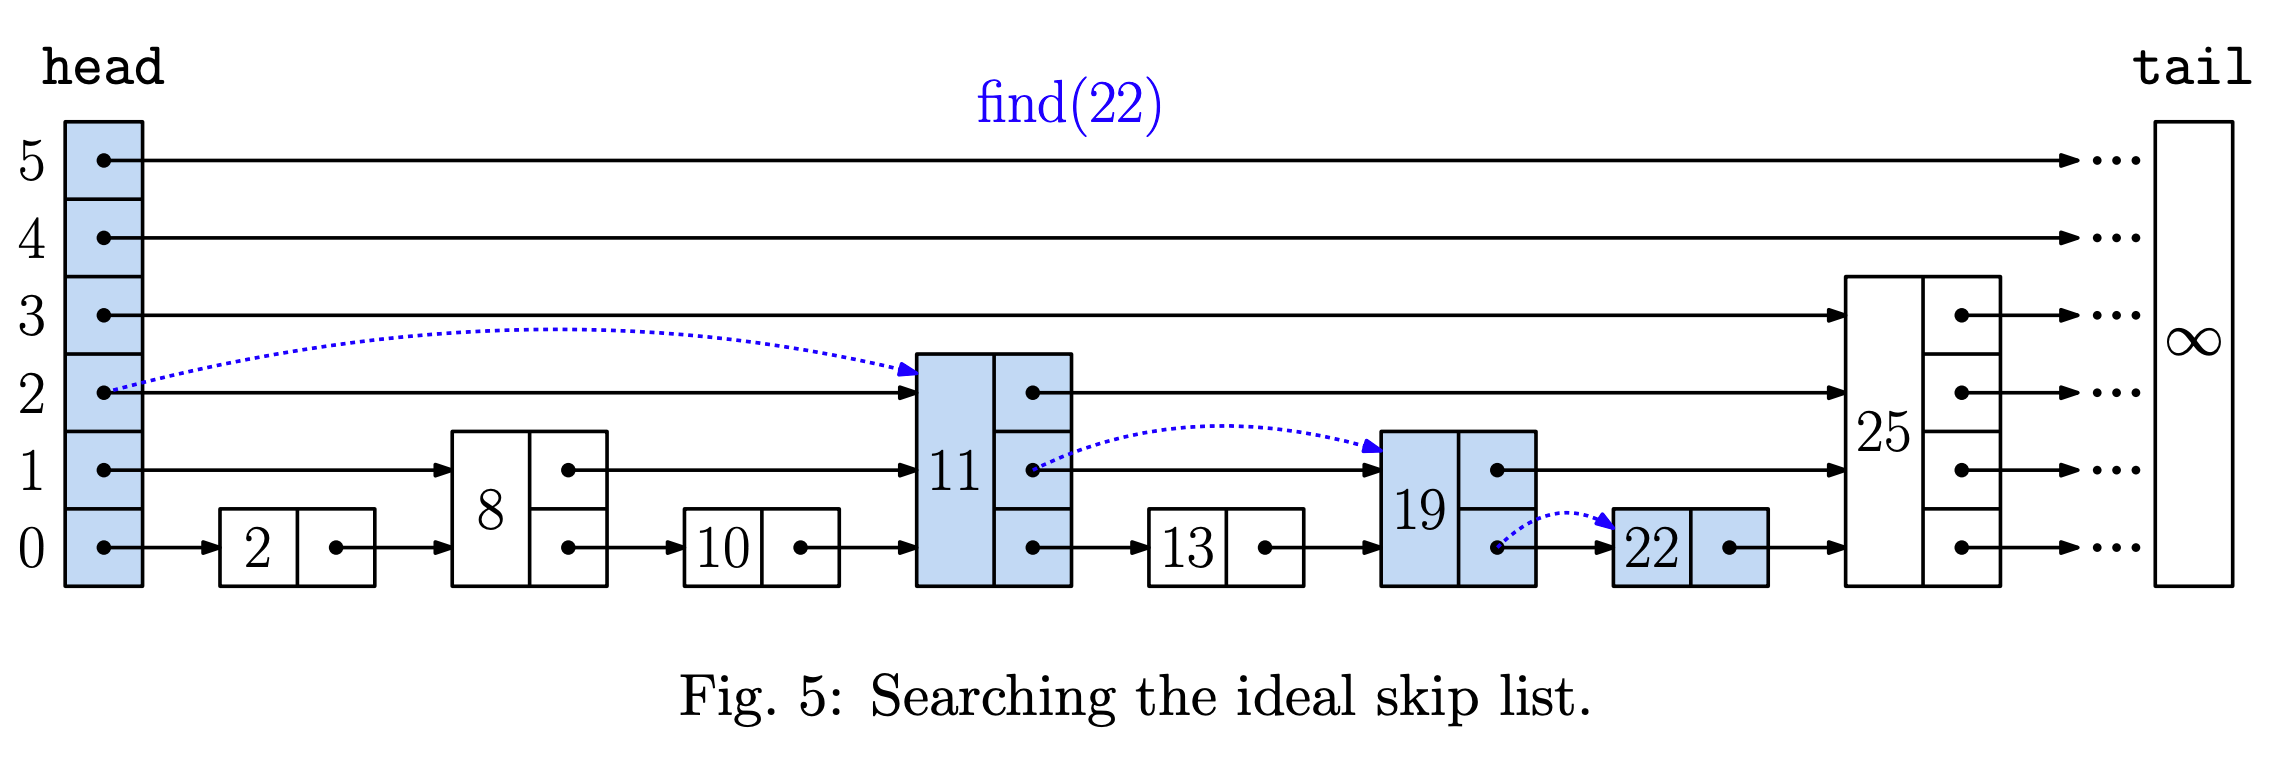
\includegraphics[width=\textwidth]{SkipListSearch}
  We can randomize the number of nodes per level by flipping a coin and only stopping at a level if tails occurs\\
  Now level k is expected to have about $\frac{n}{2^{k}}$ nodes meaning that the number of nodes at level $\ceil[\big]{lg(n)}$ is constant\\ \\
  Space Analysis: worst case every node has height log(n) so O(nlogn) total. Best each node has height 1 so O(n) total\\
  Expected Case Space: all n nodes contribute to level 0, n/2 contribute to level 1, n/4 to level 2, etc. so\\ \\
  $\sum_{i=0}^{h-1}\frac{n}{2^{i}} = n(2 - \frac{1}{2^{h}}) \leq 2n = O(n)$\\ \\
  Search Expected Runtime: for $0 \leq i \leq O(logn)$, let $E(i)$ represent the expected number of nodes visited in the skip list at the top i levels of the skip list\\
  Look at the path going backwards so it will either go up or stay on the current level and go left \\
  Whenever we arrive at some node of level i, the probability that it contributes to the next higher level is 1/2 and 1 - 1/2 to stay on same level. Counting the current node we just visited (+1) we have\\ \\
  $E(i) = 1 + \frac{1}{2}E(i-1) + \frac{1}{2}E(i) \rightarrow E(i) = 2 + E(i-1) = 2i$ by recurrence analysis and since i $\leq$ O(logn) then search is O(logn)\\ \\
  Insertion: search for x to find its immediate predecessors at each level then create node x and flip a coin until tails. Letting k denote the number of tosses made, height = min of k + 1 and height of list then link the k+1 lowest predecssors \\ \\
  Deletion: find the node and keep track of all predecessors at various level of list then unlink the target node at each level (like in standard linked list removal) \\ \\
  Implementation Notes: skip-list nodes have variable size, containing the key-value pair, variable-sized array of next pointers (p.next[i] points to the next node at level i). Also has 2 sentinel nodes (head and tail where tail.key is $\infty$ to stop search)\\
  \newpage
  \section{Splay Trees}
  Self adjusting tree that dynamically adjusts its structure according to a dynamically changing set of access probabilities
  \begin{itemize}[noitemsep]
  \item nodes that are accessed more frequently are closer to the root
  \item Binary Search Tree that uses rotations to maintain structure but doesn't need to store balance information
  \item Whenever a deep node is accessed, the tree will restructure itself so tree is more balanced 
  \item $\Omega(n)$ worst operation but amortized O(logn) \\
  \end{itemize}
  T.splay(x): searches for key x in a tree T and reorganizes T while rotating x up to the root. If x not found, use preorder predecessor or successor.
  \begin{itemize}[noitemsep]
  \item simply rotating the target node up doesn't work because it can leave the tree skewed/unbalanced
  \item instead take 2 nodes at a time and rotate both
  \end{itemize}
  For node p let parent be q and grandparent be r then
  \begin{itemize}[noitemsep]
  \item Zig-zig: if p and q are both right childnre or left children, apply rotation at r then q to bring p to the top
  \item Zig-zag: if p and q are left-right or right-left children, apply rotation to q then r to bring p to top 
  \item Zig: if p is the child of the root, rotate root of T and make p the new root
  \item if p is the root of T, we are done
  \end{itemize}
  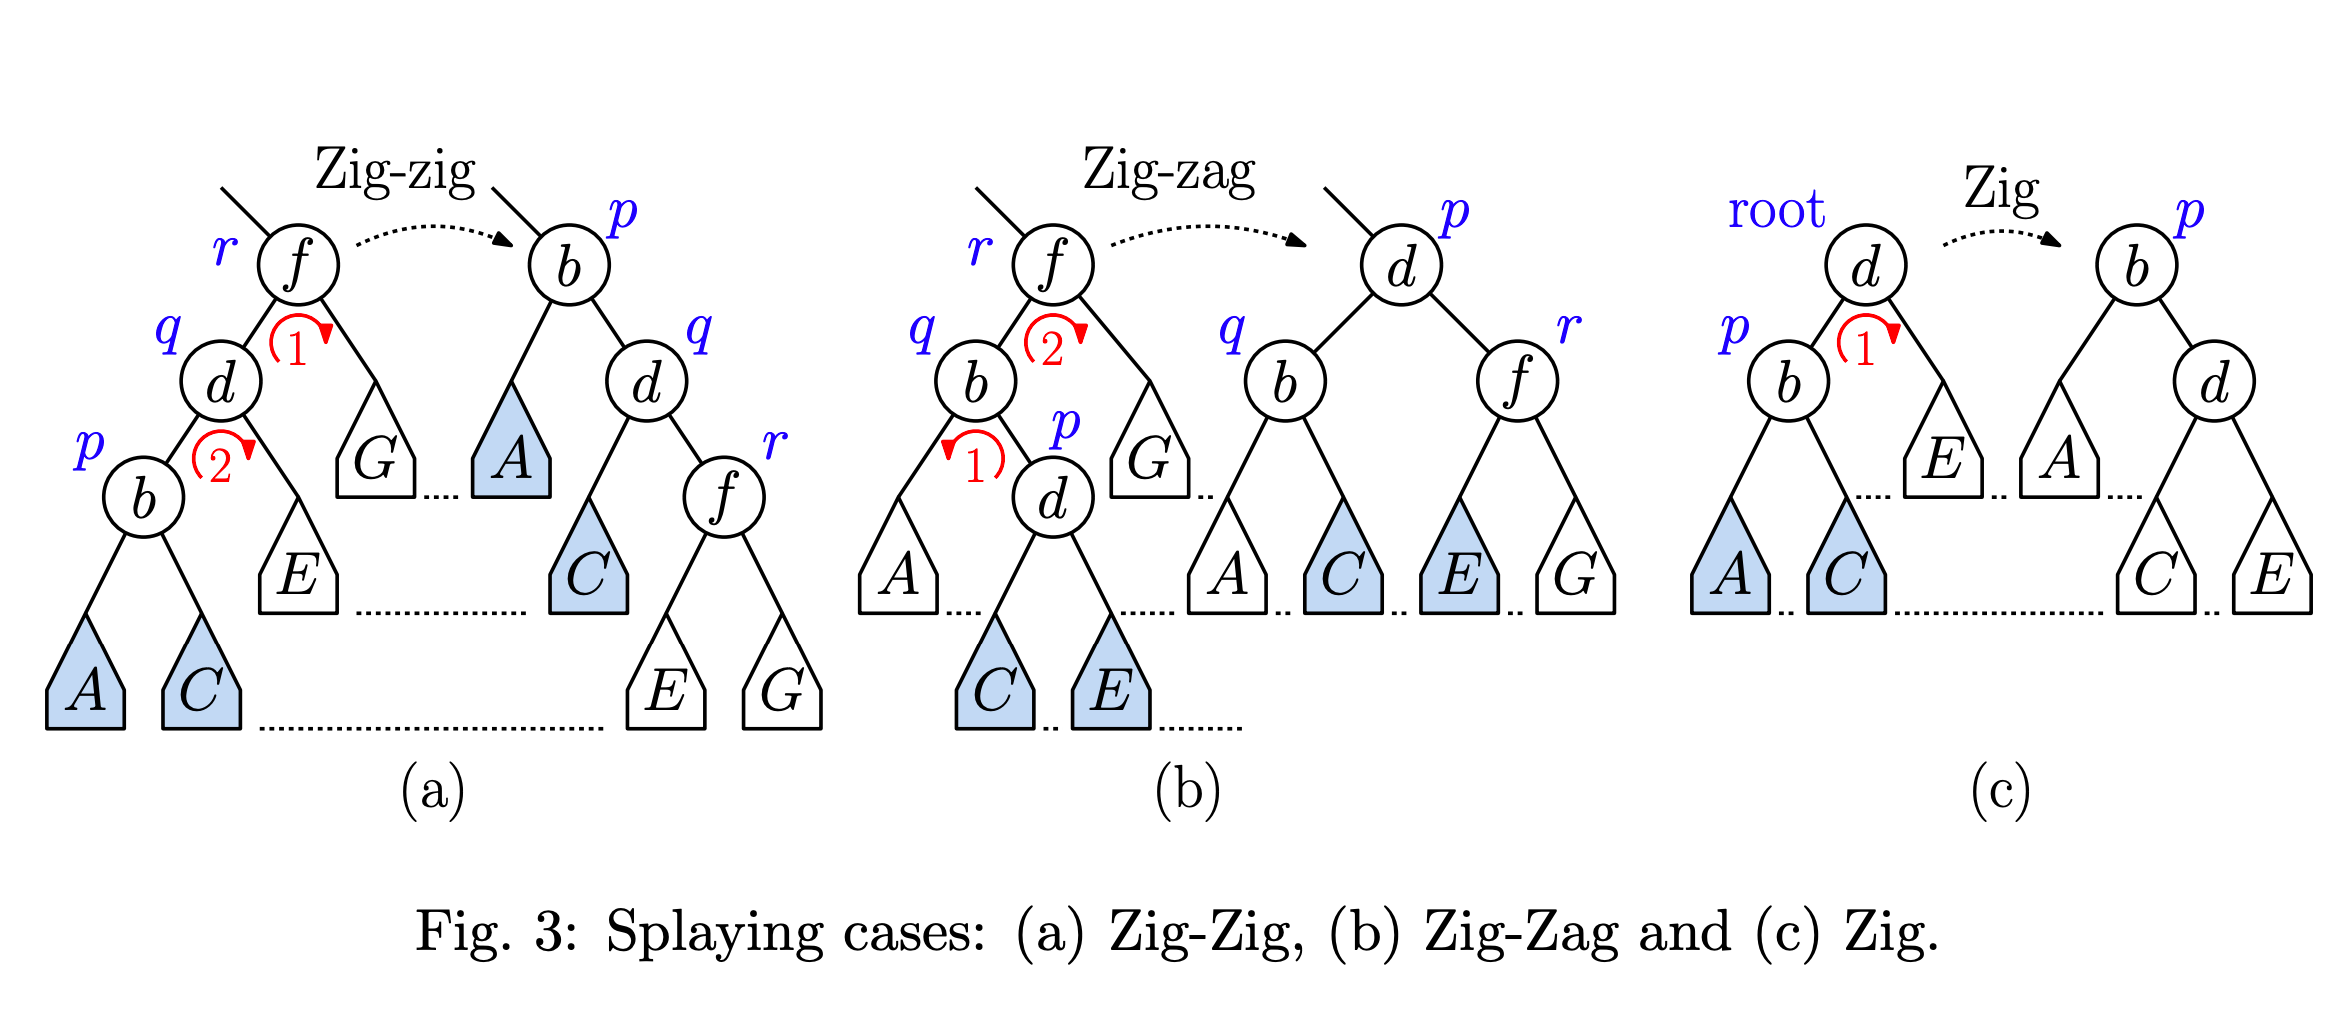
\includegraphics[width=\textwidth]{SplayTreeZig}
  Everytime zig-zig or zig-zag is called, the subtree is raised up 1 level so for a long path, these rotations will reduce its height by 1/2\\ \\
  Find: invoke T.splay(x) which transports x to the root. If root.val != x then throw an error\\ \\
  Insert(x, v): invoke T.splay(x). Let current root = y. Either
  \begin{itemize}[noitemsep]
  \item y $<$ x then all keys in R subtree $>$ x so create a new root (x,v) and add y to L and add R to new root
  \item y $>$ x then all keys in L $<$ x so create a new root (x,v) and add y to R and add L to new root
  \end{itemize}
  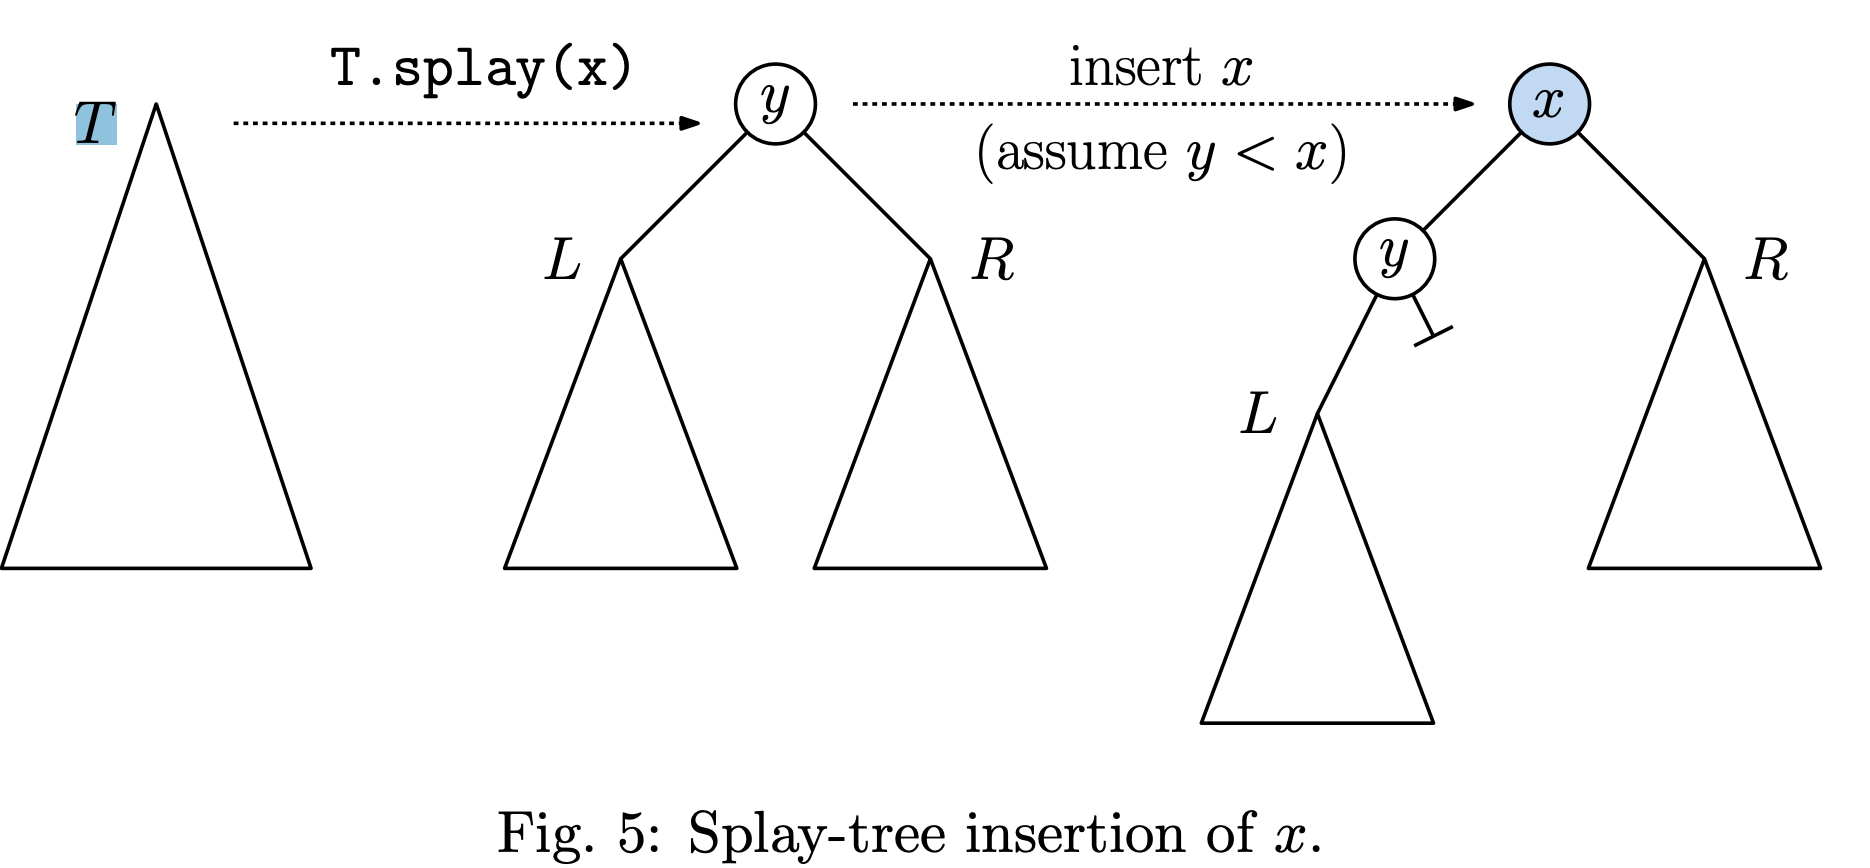
\includegraphics[width=\textwidth]{SplayInsert}
  Delete: invoke T.splay(x) then if root != x throw error. Else 
  \begin{itemize}[noitemsep]
  \item if L is empty return R
  \item if R is empty return L 
  \item Otherwise let R' = R.splay(x). This will find the inorder successor y. Since y will have no left subtree (all values in R are $>$ x), make y the new root and link L
  \end{itemize}
  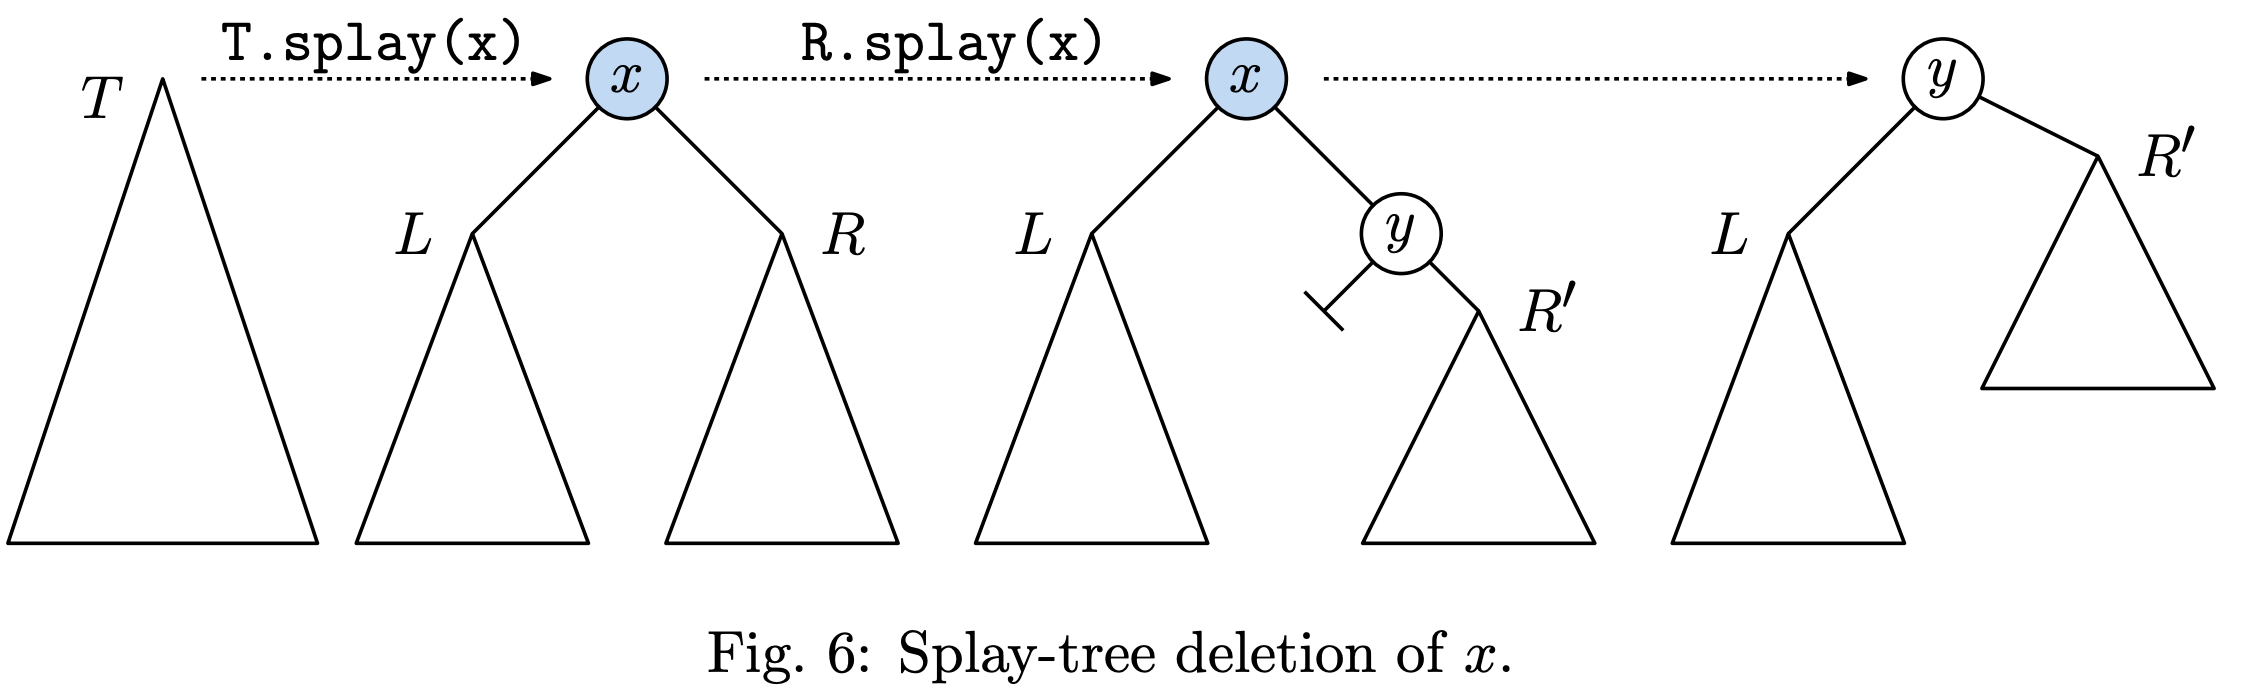
\includegraphics[width=\textwidth]{SplayDelete}
  \newpage
  \section{B-Trees}
  J-ary multiway search trees where each node stores reference to j subtrees $T_{1}, T_{2}, ..., T_{j}$ and has j-1 keys $a_{1} < a_{2} < a_{j-1}$ such that each $T_{i}$ subtree stores nodes whos keys are $> a_{i-1}$ and $< a_{i}$\\ 
  Achieves balance by constraining width of each node \\
  For any int m $\geq$ 3, B-tree of order m is a multiway search tree if: 
  \begin{itemize}[noitemsep]
  \item root is leaf or has $2 \leq x \leq m$ children
  \item each node except root has between $\ceil[\Big]{\frac{m}{2}}$ and m children which can be null
  \begin{itemize}[noitemsep]
    \item node with j children has j-1 keys
  \end{itemize}
  \item All leaves are on the same level of the tree \\
  \end{itemize}
  Height Analysis: as B-Trees grow wider, the height decreases\\
  B-Tree of order m with n keys has height of at most $(lgn)/\gamma$ where $\gamma$ = lg(m/2)\\
  Proof: assume m is even and let N(h) = number of nodes in skinniest possible order-m B tree of height h\\
  \indent Root has $\geq$ 2 children that have $\geq$ m/2 children \\
  \indent \indent therefore 2 nodes at depth 1\\
  \indent \indent $2(m/2)$ nodes at depth 2\\
  \indent \indent $2(m/2)^{2}$ nodes at depth 3\\
  \indent \indent $2(m/2)^{k-1}$ nodes at depth k\\
  \indent So $N(h) = \sum_{i=1}^{h}2(\frac{m}{2})^{i-1}$\\
  \indent let c = m/2\\
  \indent $N(h) = \frac{2(c^{h}-1)}{(c-1)} \approx \frac{2c^{h}}{c} = 2c^{h-1} = 2(\frac{m}{2})^{h-1}$\\
  \indent Each node has $\geq \frac{m}{2}-1$ keys $\approx \frac{m}{2}$\\
  \indent $n \geq N(h) \geq 2(\frac{m}{2})^{h} \rightarrow h \leq \frac{lgn}{lg\frac{m}{2}}$\\ \\
  Node Structure: since B-Tree nodes can hold a variable number of items, every node is allocated max possible size
  \begin{lstlisting}
    final int M = m;    \\order of B-tree
    class BTreeNode {
      int nChildren;
      BTreeNode child[M];
      Key key[M-1];
      Value value[M-1]; 
    }
  \end{lstlisting}
  Searching: When arriving at an interval node, search through keys
  \begin{itemize}[noitemsep]
  \item if x is found then return the corresponding value
  \item Else determine index i such that $a_{i-1} < x < a_{i}$ note that $(a_{0} = -\infty, a_{j} = \infty)$
  \item Then recurse into subtree $T_{i}$\\
  \end{itemize}
  Insertion and Deletion require some restructuring methods (rotation, splitting, and merging)\\ \\
  Rotation: Node can have between $\ceil[\Big]{m/2}$ and $m$ children, and one less keys. Insertion and deletion might make a node have too many or too few nodes so we fix this imbalance by moving a child into or from one of its siblings, assuming the sibling isn't full\\
  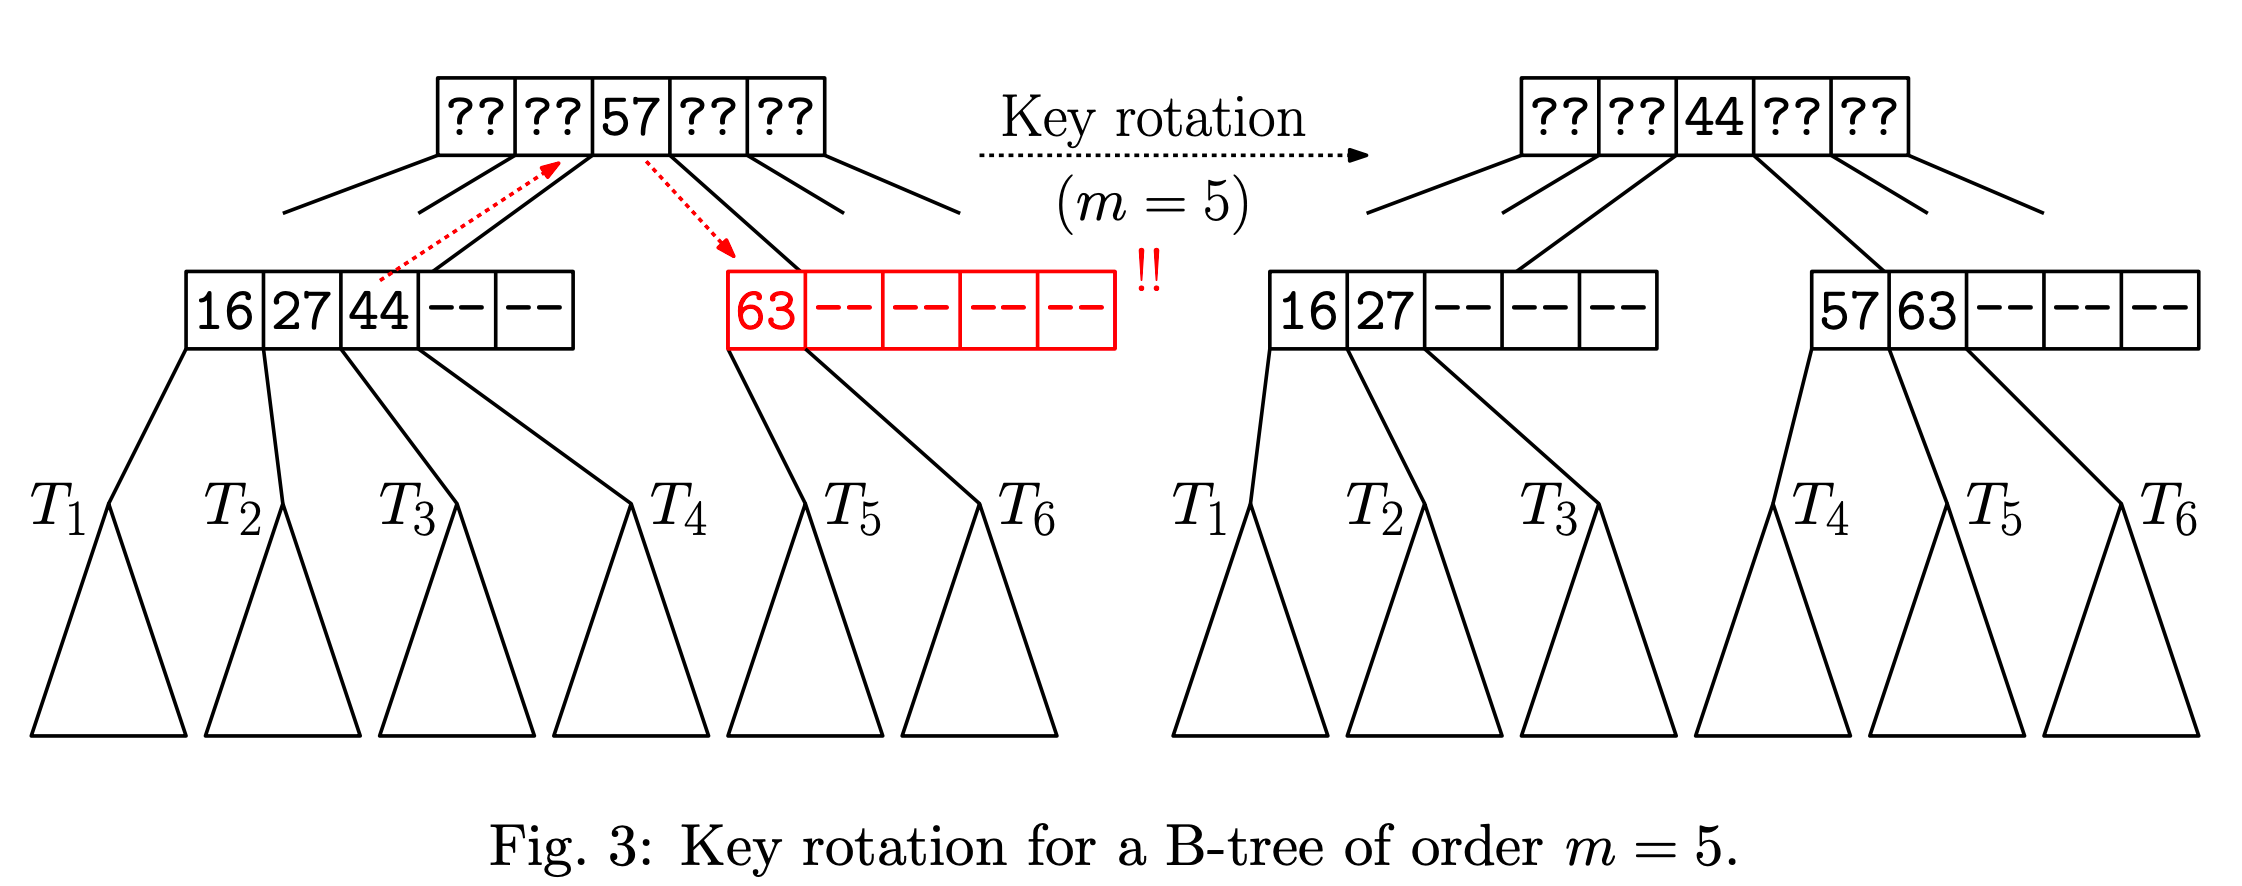
\includegraphics[width=\textwidth]{BTreeRotations}
  Node Splitting: node has 1 too many children (m + 1 children and m keys) and key rotation is not available so split node into 2 nodes, one with $m' = \ceil[\Big]{m/2}$ children and the other with $m''= m + 1 - \ceil[\Big]{m/2}$ children\\
  Since $(m' - 1) + (m'' - 1) = m - 1$, we have one extra key that is doesn't fit into L and R subchildren so it is promoted to parent and then handled up there\\
  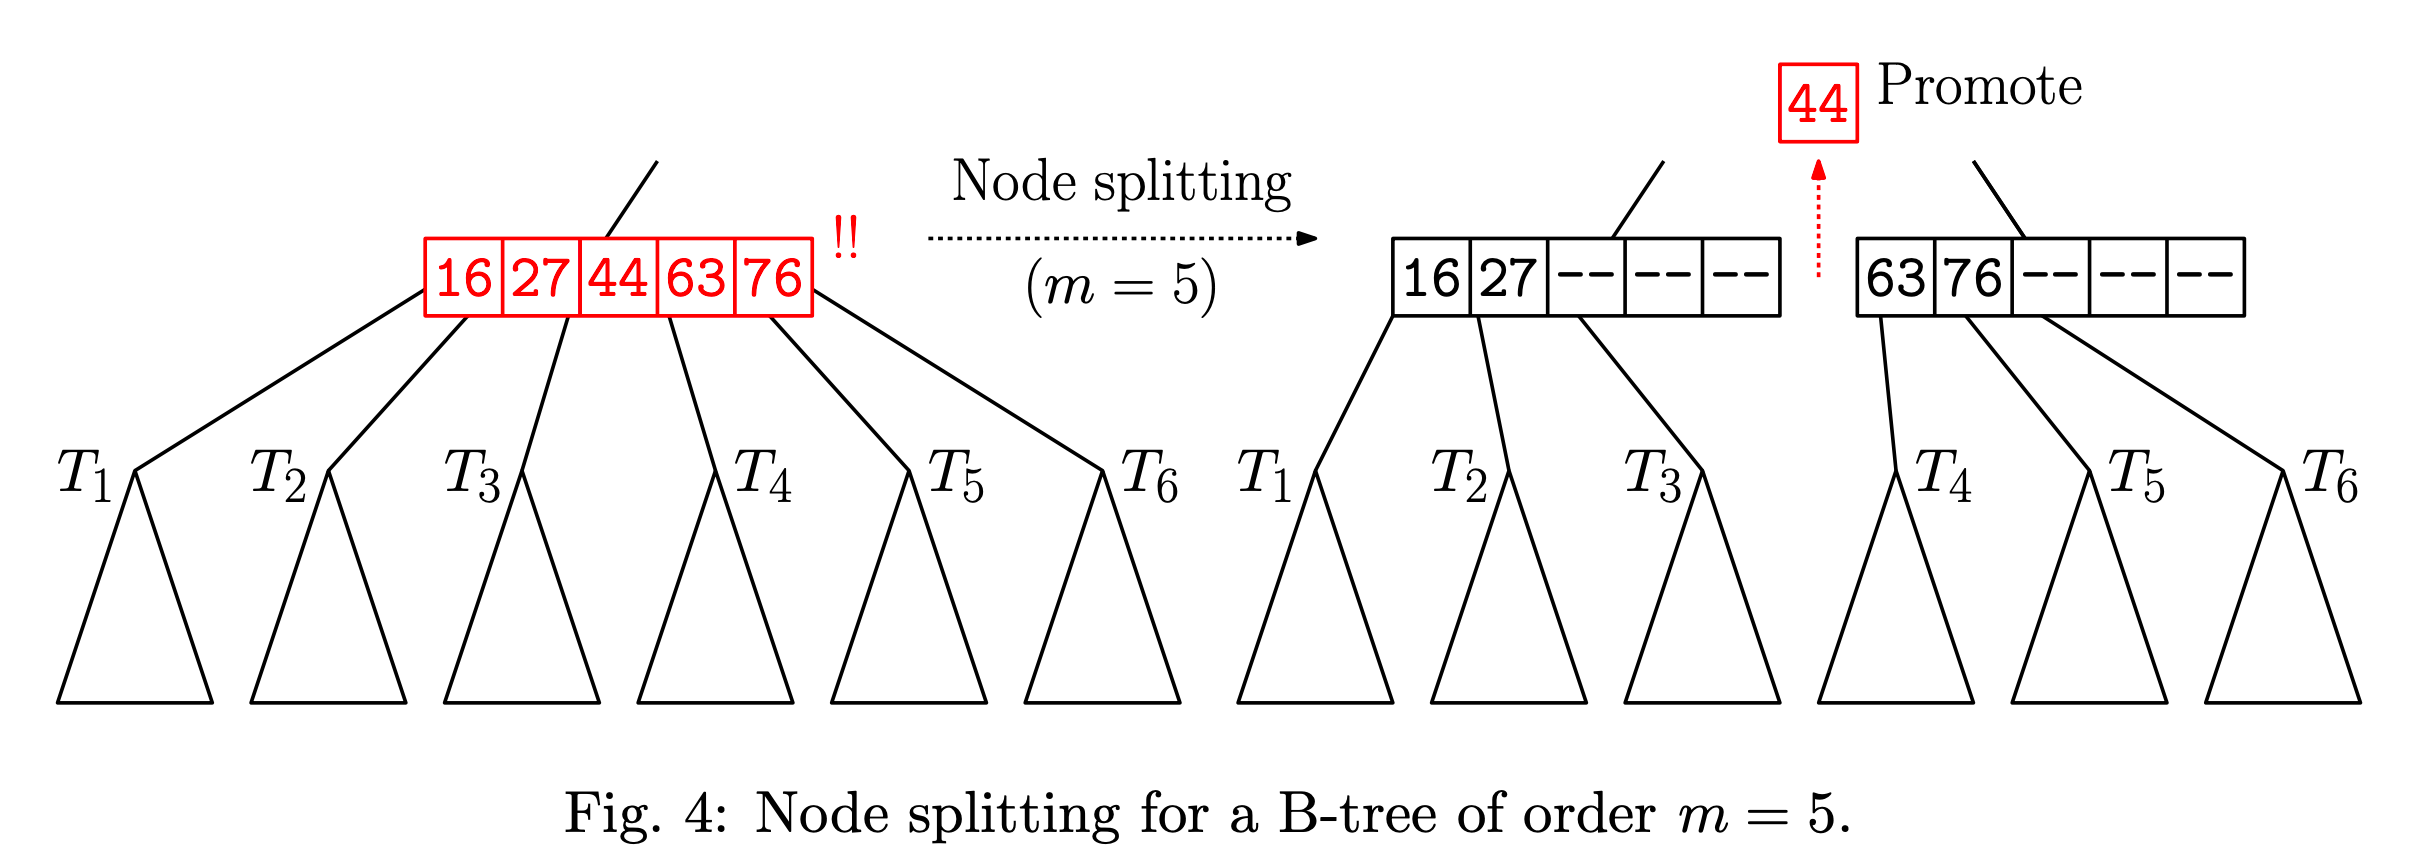
\includegraphics[width=\textwidth]{BTreeNodeSplitting}
  Proof for Node Splitting:
  \begin{itemize}[noitemsep]
  \item If m is even then $\frac{m}{2} \leq m + 1 - \frac{m}{2} = \frac{m}{2} + 1 \leq m$
  \item If m is odd then $\frac{m+1}{2} \leq m + 1 - \frac{m+1}{2} = \frac{m+1}{2} \leq m$ \\
  \end{itemize}
  Node Merging: Node might have 1 too few children ($\ceil[\Big]{m/2} - 1$ nodes and one less keys) after deletion. If key rotation isn't available, then we know that the sibling must have the minimum number of children $(\ceil[\Big]{m/2})$. Now merge node with the sibling into a node with $m' = (\ceil[\Big]{m/2} - 1) + \ceil[\Big]{m/2} = 2\ceil[\Big]{m/2} - 1$ children\\
  Note that $\ceil[\Big]{m/2} - 2 + \ceil[\Big]{m/2} = m' - 2$ which is one too few so we demote the appropriate key from the parent's node to get desired number of keys. \\
  Since the parent lost a key and a node, recurse up to parent\\ \\
  Lemma: For all $m \geq 2$, $\ceil[\Big]{m/2} \leq 2\ceil[\Big]{m/2} - 1 \leq m$
  \begin{itemize}[noitemsep]
  \item If m is even then $\frac{m}{2} \leq m - 1 \leq m$
  \item If m is odd then $\frac{m+1}{2} \leq m \leq m$
  \end{itemize}
  \includegraphics[width=\textwidth]{BtreeNodeMerge}
  Insertion: creating nodes is an expensive operation so try to rotate whenever possible. Search for key x and if
  \begin{itemize}[noitemsep]
  \item found thrown an exception
  \item leaf is not at full capacity (fewer than m-1 keys) then we insert key and done
    \begin{itemize}[noitemsep]
      \item may involve sliding around but can ignore the cost since m is constant
    \end{itemize}
  \item otherwise node overflows and check if either sibling is less than full. If so then perform a rotation else perform node split. 
  \end{itemize}
  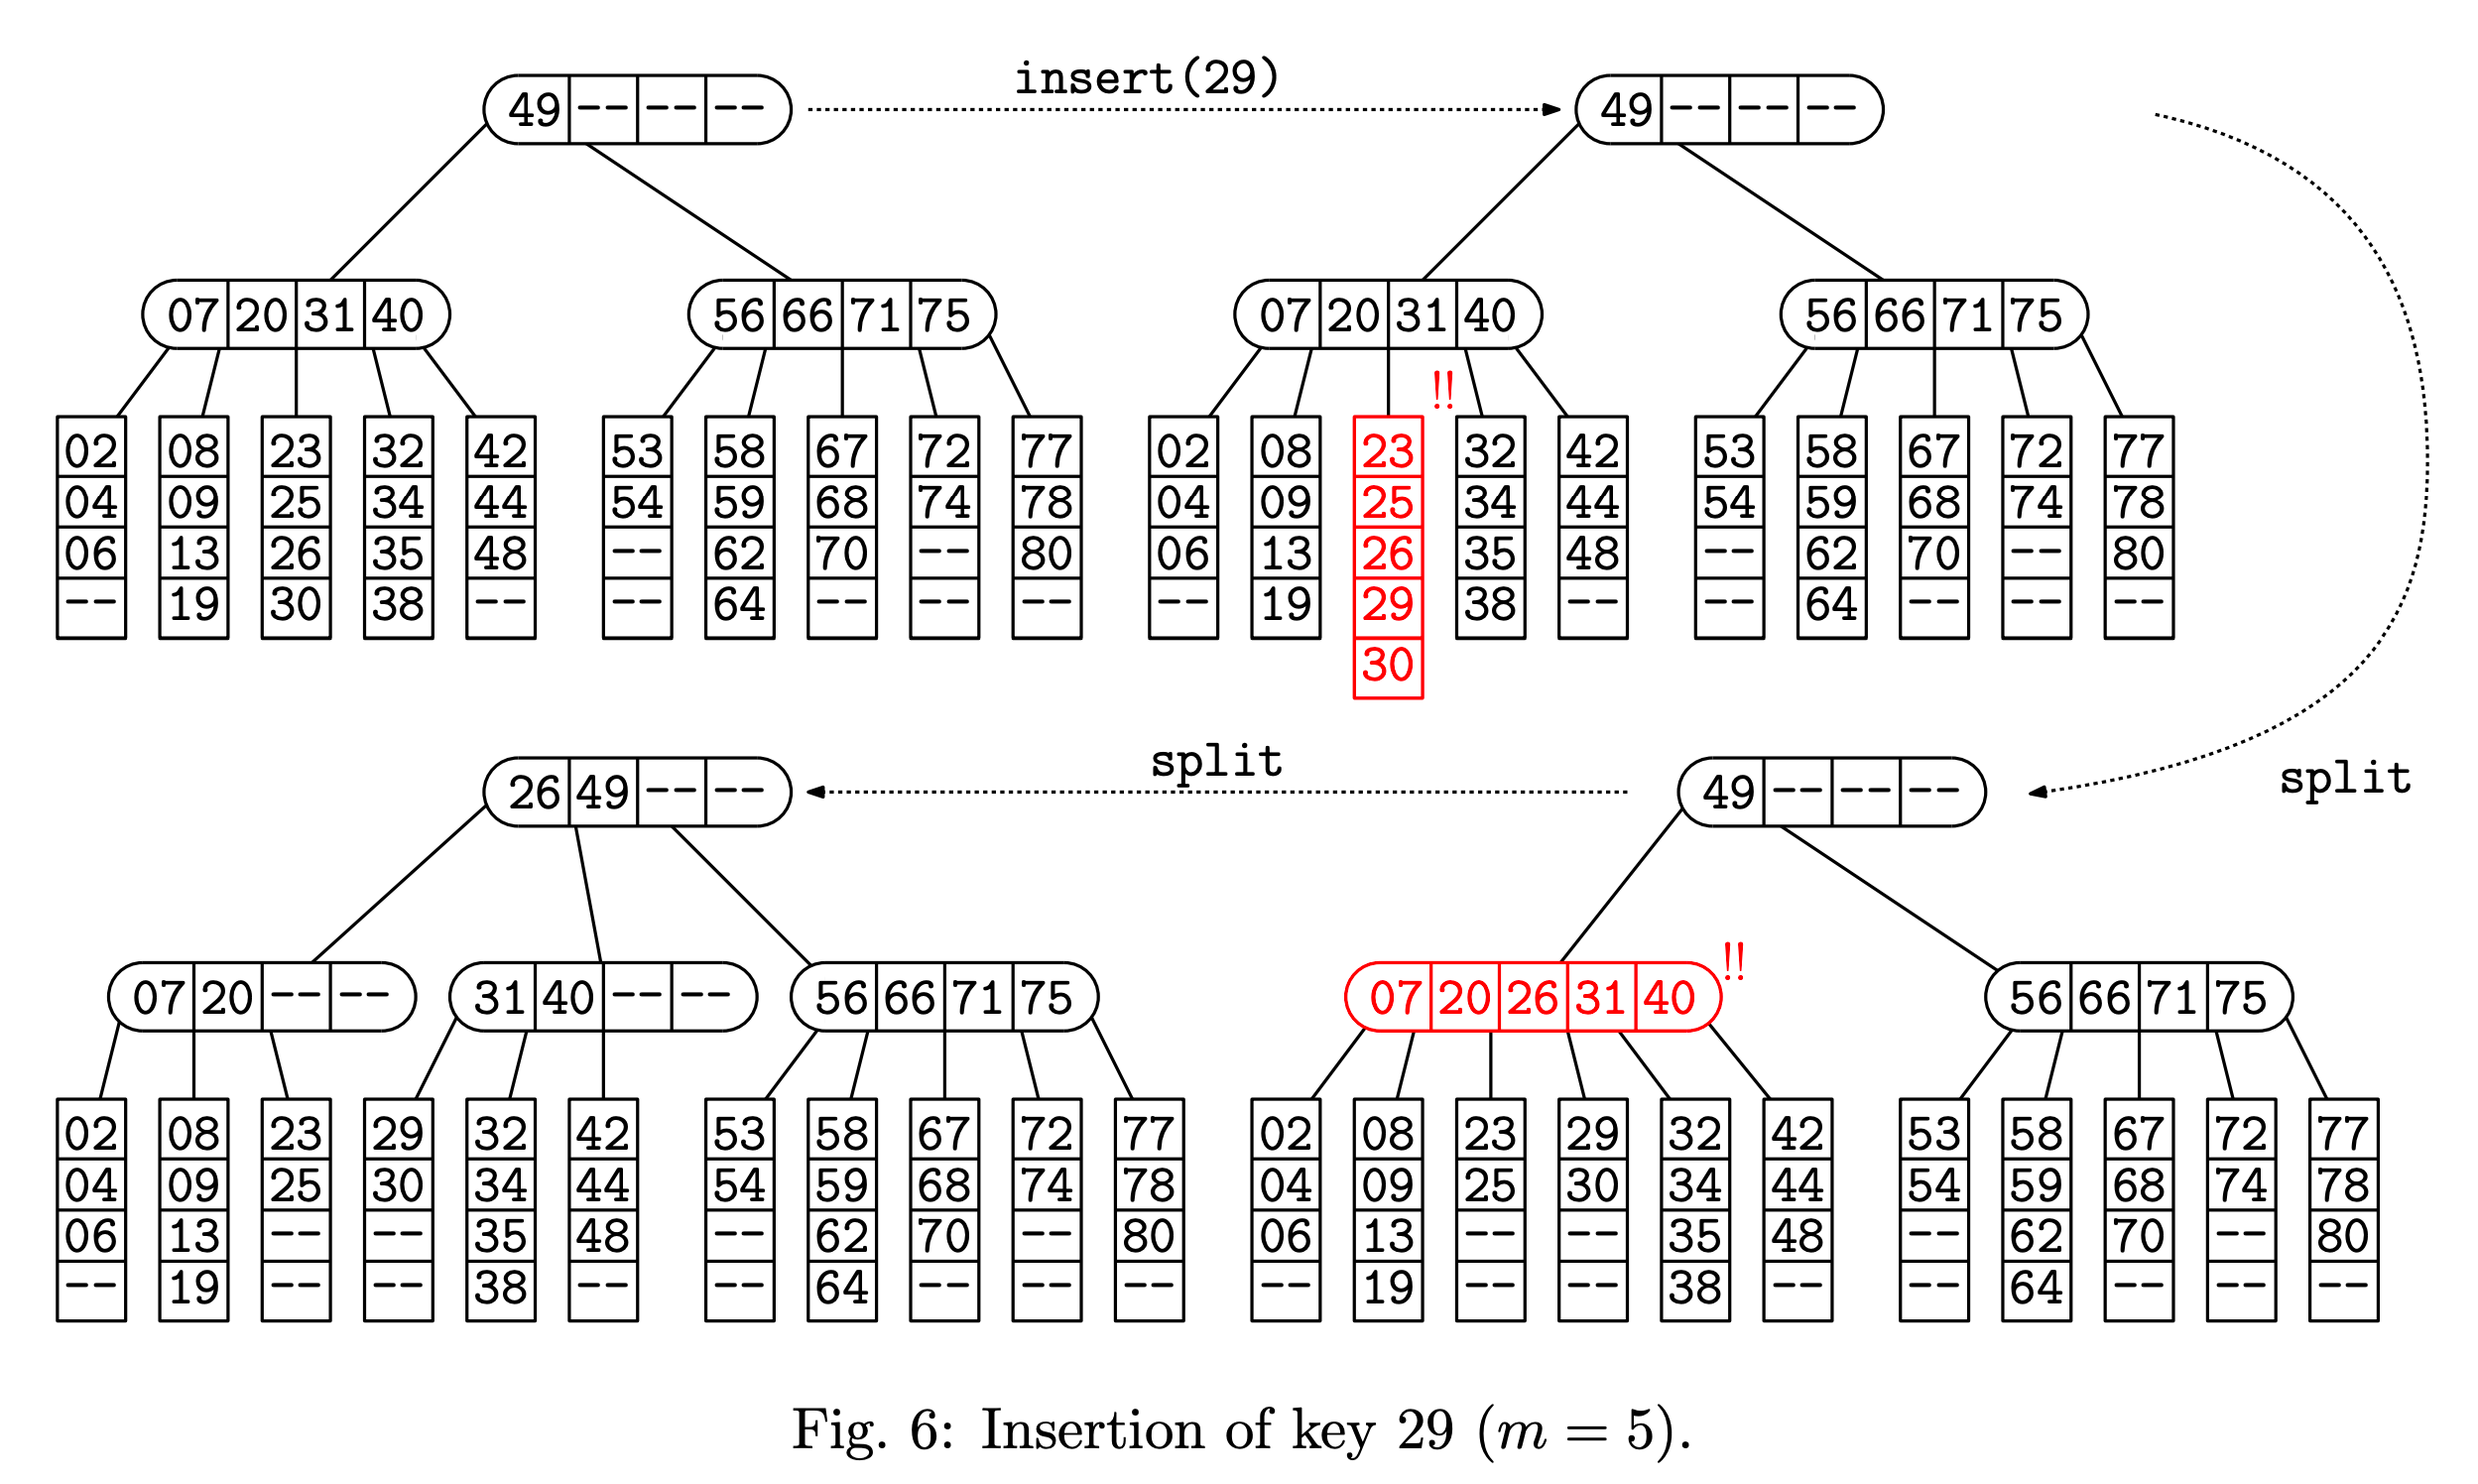
\includegraphics[width=\textwidth]{BTreeInsertion}
  \newpage
  Deletion: Search for the node to be deleted. Need to find replacement so take largest key in left child or smallest key in right child and move this key up to fill the hole
  \begin{itemize}[noitemsep]
  \item if left node has $\geq \ceil[\Big]{m/2} - 1$ keys we are done
  \item else node will underflow so key rotate if possible else use node merge and recurse in parent
  \end{itemize}
  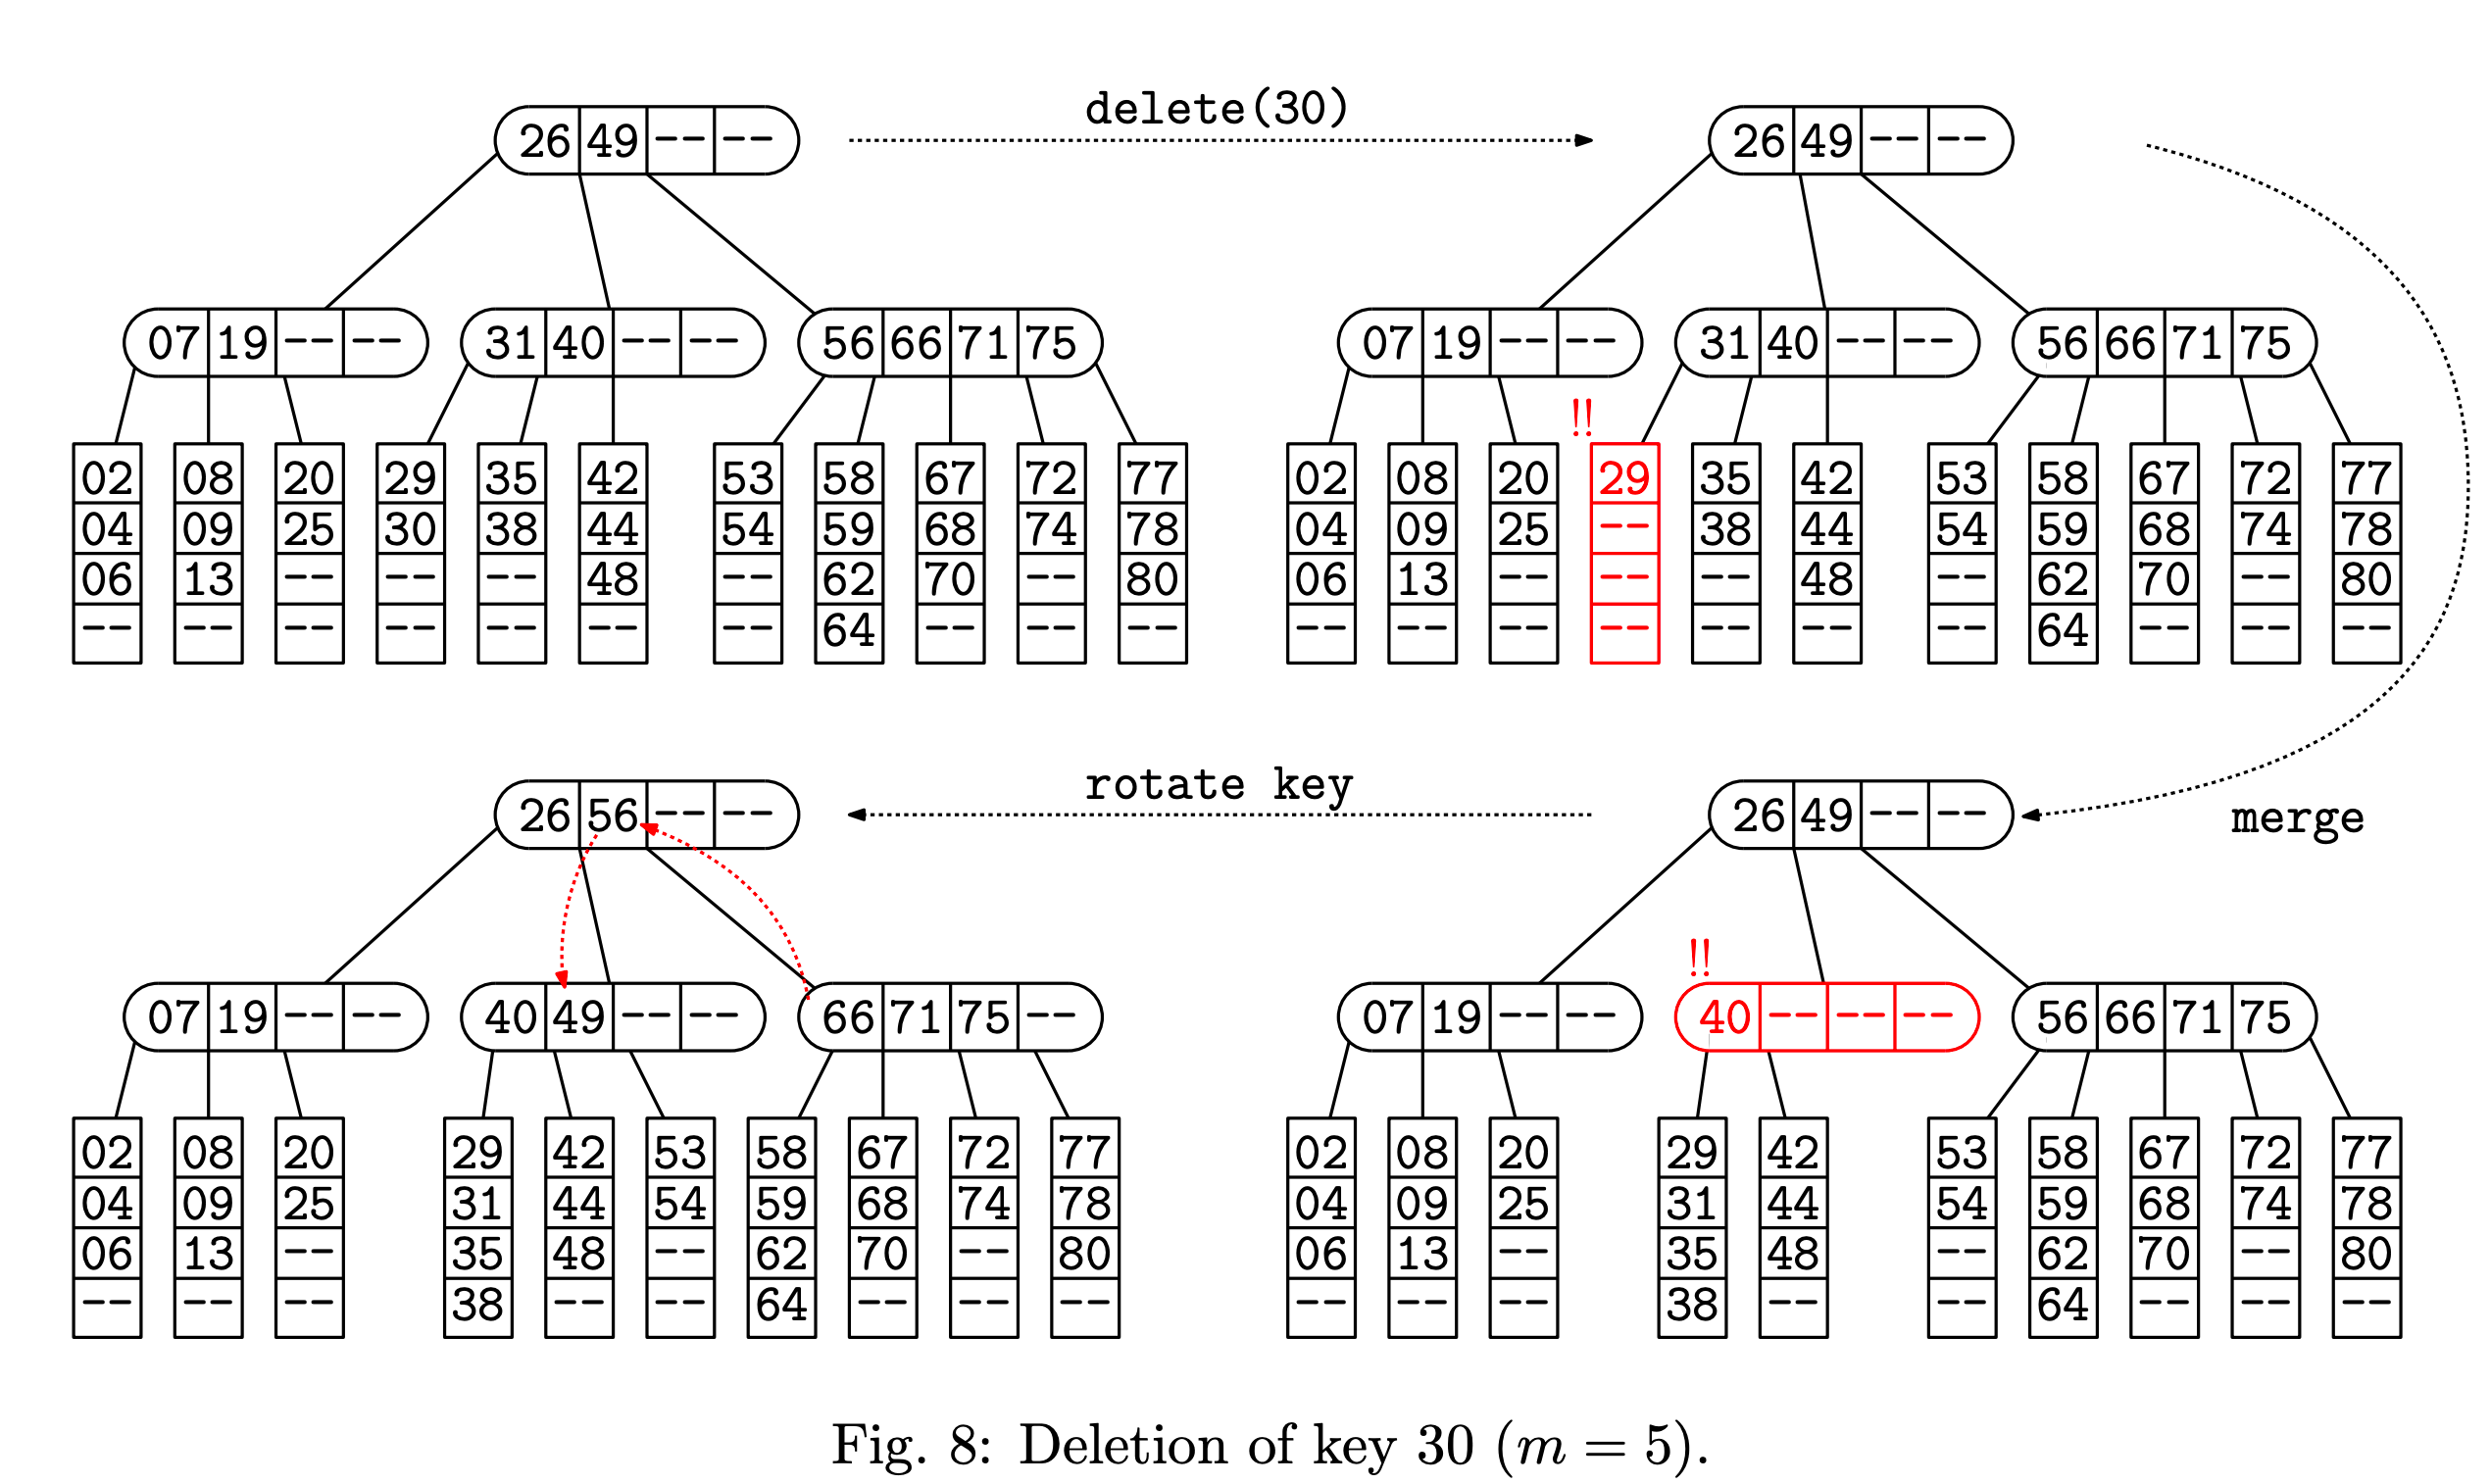
\includegraphics[width=\textwidth]{BTreeDeletion}
  B+ Trees: internal nodes only store keys (not values)\\
  Keys are used solely for locating leaf node containing actual data so it's not necessary that every key in internal node to correspond to a key-value pair\\
  Each leaf node has a next-leaf pointer, which pointers to the next leaf in sorted order \\
  Storing only in internal nodes save space and allows increased tree fan out $\rightarrow$ lowers height ofr tree\\
  Internal nodes are an index to locate actual data which resides at the leaf level\\
  Now internal nodes with keys $a_{1}, ..., a_{j-1}$, subtree $T_{j}$ has keys x such that $a_{i-1} < x \leq a_{i}$\\
  Next leaf enables efficient range reporting quries where we can list keys in range $[x_{min}, x_{max}]$\\
  \indent so we now find the leaf node $x_{min}$ and follow next leaf links until we reach $x_{max}$\\
  \newpage
  \section{Hashing}
  Supports O(1) dictionary operations but cannot perform search operations like range queries (finding keys x such that $x_{1} \leq x \leq x_{2}$) or nearest-neighbor queries (find key closest to a given key x)\\
  Given a table of size m > n and a hash function h(x), we use h(x) to map a key to a random index $[0...m-1]$ \\
  Possible issue of collisions where 2 keys land in the same index after hashing\\ \\
  Good hash function:
  \begin{itemize}[noitemsep]
  \item Efficiently computable
  \item Produces few collisions
    \begin{itemize}[noitemsep]
      \item function on every bit of key 
      \item scatters naturally occuring clusters of keys \\
    \end{itemize}
  \end{itemize}
  Types of hasing:
  \begin{itemize}[noitemsep]
  \item Division Hashing: $h(x) = x mod m$
    \begin{itemize}[noitemsep]
      \item Fails 2nd rule (issue with clusters)
    \end{itemize}
  \item Multiplicative Hashing: $h(x) = (ax) mod m$
  \begin{itemize}
    \item Where a is a large prime number
  \end{itemize}
  \item Linear Hashing: $h(x) = (ax + b) mod m$
  \begin{itemize}
      \item Enhances Multiplicative hashing with added constant
  \end{itemize}
  \item Polynomial Hashing: $h(x_{0}, ..., x_{n}) = (\sum_{i=0}^{k-1}c_{i}p^{i}) mod m$
    \begin{itemize}
      \item Useful for keys that have a sequence of objects (strings or coordinates)
      \item Can use Horner's Rule to make summation faster $c_{0} + c_{1}p + c_{2}p^{2} + c_{3}p^{3} = ((c_{3}p + c_{2})p + c_{1})p + c_{0}$ \\
    \end{itemize}
  \end{itemize}
  Universal Hashing: hash function is selected from large class of functions so probability of collision between 2 fixed keys is about 1/m\\
  Consider a large prime $p$ and two random integers $a \in \{1, 2, ..., p-1\}$ and $b \in \{0, 1, ..., p-1\}$ \\
  Use a linear has function $h_{a,b}(x) = ((ax + b) mod p mod m$. As a and b vary, they will define a family of functions.\\
  Let $H_{p}$ denote the class of hash functions that arise from all possible combos of a and b. If we consider any two integers x and y such that $0 \leq y < x < p$ then the probability $h_{a,b}(y) = h_{a,b}(x)$ is 1/m\\ \\
  Handling Collisions Separate Chaining: have each index be a linked list and store collisions by adding to these linked lists.
    \begin{itemize}[noitemsep]
    \item We define the load factor $\lambda = n/m$ and expect each list to have about $\lambda$ elements
    \item If we are successful in finding the desired element, it'll take about $1 + \frac{\lambda}{2}$ (about halfway). Otherwise failure will take $1 + \lambda$. Additional 1 is for null checks
    \item Insertion and deletion will take about constant time so all dictionary operations will take $O(1 + \lambda)$
    \item Drawback of we need to use additional storage to store pointers to linked lists
    \end{itemize}
  Controlling Load Factor and Rehashing: we want to maintain a few invariants
  \begin{center} 
    $0 < \lambda_{min} < \lambda_{max} < 1$ \quad $\lambda_{min} \leq \lambda \leq \lambda_{max}$ \quad $n \leq \lambda_{max}m$ \quad $m \leq n/\lambda_{min}$
  \end{center}
  We don't want too large of a table or too small of a table so the optimal load factor is $\lambda_{0} = (\lambda_{max} + \lambda_{min}) / 2$\\
  If load factor is too big ($n > lambda_{max}m$) or too small ($n < \lambda_{min}m$) then we rehash with a larger table
  \begin{itemize}
    \item Allocate a table of size $m' = \ceil{n/\lambda_{0}}$
    \item generate new hash function $h'$ using new table size
    \item Insert every entry from old table to new table using new hash function
    \item remove old table
    \item New load factor ($n/m'$) $\approx \lambda_{0}$ so we have restored optimal load factor
  \end{itemize}
  Amortized cost of rehashing is still good since we only rehash every so often \\ \\
  Open Addressing: To know which table entries have values and which are empty we store a special value \textit{empty}. Now whenever we insert an element and its hashed index is already occupied we probe around nearby entries until we find an empty slot. The secondary search involves a function $f$ so now the probe sequence is
  \begin{center}
    $(h(x) + f(1)) mod m, (h(x) + f(2)) mod m, ...$
  \end{center}
  \newpage
  Linear Probing: probe function is $f(i) = i$ and we search sequential locations until we find an empty slot
  \begin{itemize}[noitemsep]
    \item good for low load ($<75\%$)factor. As load factor approaches 1, becomes very bad
    \item Issue with secondary clustering (when keys has to different locations but collision-resolution results in new collisions)
    \item Successful search expected cost: $(\frac{1}{2}(1 + \frac{1}{1 - \lambda}))$ \quad Unsuccessful serach expected cost: $(\frac{1}{2}(1 + (\frac{1}{1 - \lambda})^{2}))$ \\
  \end{itemize}
  Quadratic Probing: Avoids secondary clustering by using a nonlinear probing function, scattering subsequent probes. Example Code:
  \begin{lstlisting}
    Value find(Key x) {
      int c = h(x);
      int i = 0;
      while ((table[c].key != empty) && (table[c].key != x)){
        c += 2*(++i) - 1;
        c = c \% m
      }
      return table[c].value;
    }
  \end{lstlisting}
  Quadratic Probing has a potential issue of skipping potential slots due to growth factor. However if m is prime, we can guarantee that $\ceil{m/2}$ probe sequences are distinct. Proof:\\
  Contradiction: assume $0 \leq i < j \leq \ceil{m/2}$ then \\
  $h(x) + i^{2} \equiv h(y) + j^{2} \iff i^{2} \equiv j^{2} \equiv i^{2} - j^{2} \equiv 0 \iff (i-j)(i+j) \equiv 0 mod m$ but its impossible since m is prime\\
  Other cool properties:
  \begin{itemize}[noitemsep]
    \item if $m = 4k + 3$ and is prime, then quadratic probe will work for all table entries before repeating
    \item if m is a power of 2 and the increment factor is $\frac{1}{2}(i^{2} + i)$ then we can probe every table entry before repeating \\
  \end{itemize}
  Double Hashing: use a hash function to figure out the probe sequence $f(i) = i*g(x)$. Now
  \begin{center} 
    $h(x) + g(x), h(x) + 2g(x), h(x) + 3g(x), ...$
  \end{center}
  To ensure that there are no cycles, $m$ and $g(x)$ must be relatively prime\\
  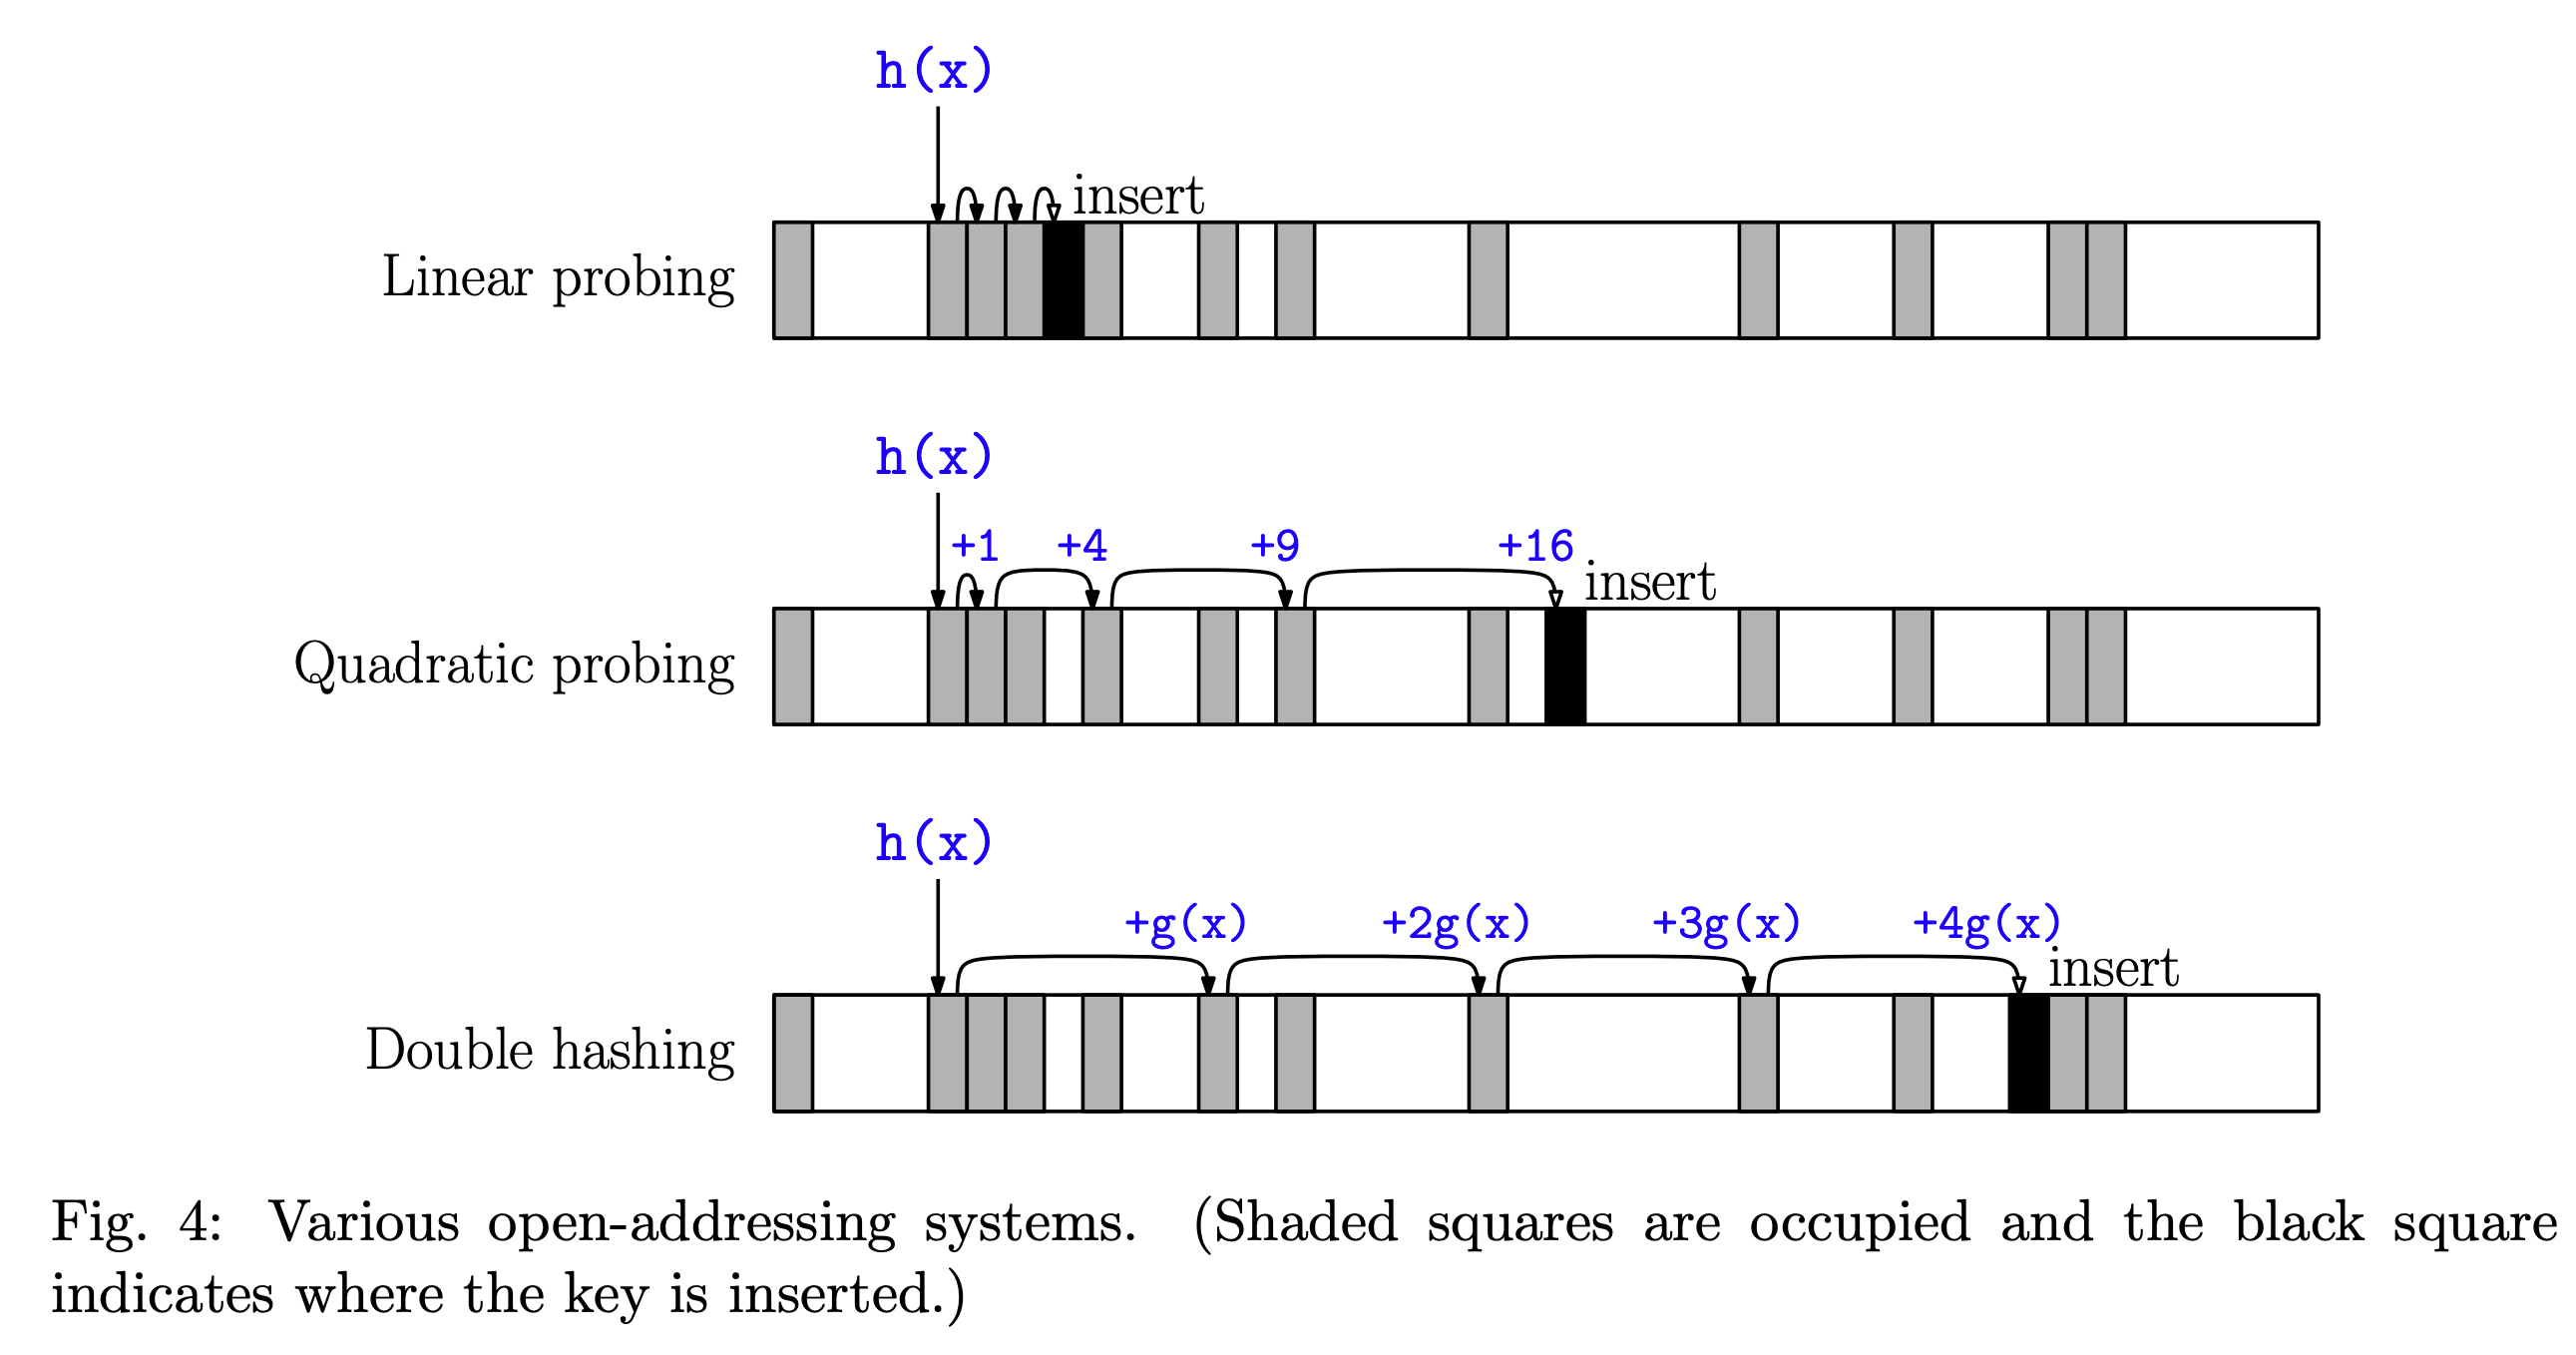
\includegraphics[width=\textwidth]{HashProbe}
  Successful search expected cost: $(\frac{1}{\lambda}\ln(\frac{1}{1 - \lambda}))$ \quad Unsuccessful serach expected cost: $(\frac{1}{1 - \lambda})$ \\ \\
  Deletition can be tricky since if we delete a node in the probe sequence, we cannot find the latter elements in that probe sequence. To resolve this, we create a special value called \textit{deleted} meaning that that slot is available for insertion but search method can continue searching the probe sequence until it finds the target element or reaches an empty cell \\
  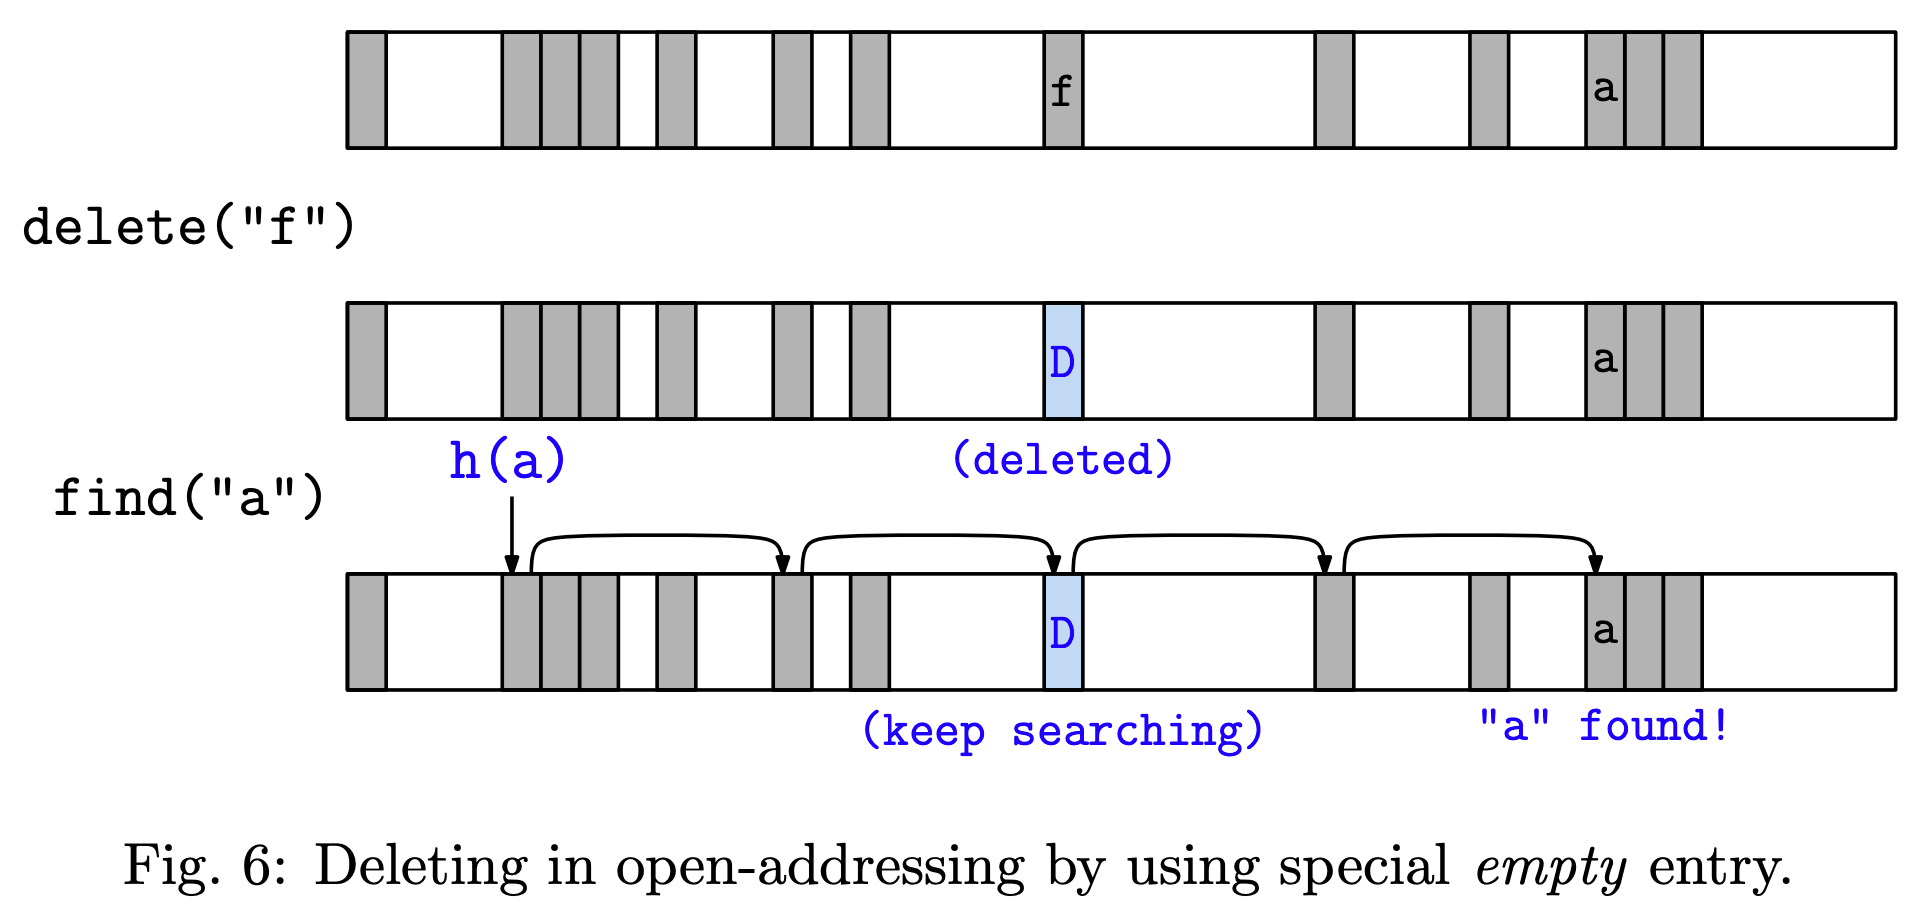
\includegraphics[width=\textwidth]{HashDeletion}
  However, this solution makes can make the search path extremely long (even if the load factor is low). Another possible solution is to bring up the latter elements of the probe sequence up after deleting an element, but that makes deletion take longer.\\
\end{document}

